\documentclass[a4paper]{report}


\usepackage{amsmath, amssymb, amsthm}
\usepackage{mathtools}
\usepackage{proof}
\usepackage{bussproofs}
\usepackage{color}
\usepackage{geometry}
\usepackage{enumerate}
\usepackage{extarrows}
\usepackage{verbatim}
\usepackage[ampersand]{easylist}
\usepackage[linewidth=1pt]{mdframed}
%\usepackage{tcolorbox}
\usepackage[font=large,labelfont=bf]{caption}
\usepackage{float}

\geometry{left=2.5cm,right=2.5cm,top=2.5cm,bottom=3cm}

\renewcommand\qedsymbol{$\blacksquare$}

\newtheorem{thm}{Theorem}[chapter]
\newtheorem{lem}[thm]{Lemma}
\newtheorem{defi}[thm]{Definition}
\newtheorem{nota}[thm]{Notation}
\newtheorem{prop}[thm]{Proposition}
\newtheorem{cor}[thm]{Corollary}

\newtheorem{example}{Example}[chapter]


\usepackage{listings}
\definecolor{blue}{rgb}{0.0, 0.0, 1.0}
\definecolor{lbcolor}{rgb}{0.9,0.9,0.9}
\definecolor{darkgreen}{rgb}{0.0, 0.42, 0.24}
\definecolor{darkblue}{rgb}{0,0,1}
\definecolor{daffodil}{rgb}{1.0, 1.0, 0.19}
\definecolor{coolblack}{rgb}{0.0, 0.18, 0.39}
\definecolor{carnelian}{rgb}{0.7, 0.11, 0.11}
\definecolor{gray}{rgb}{0.3,0.3,0.3}
\definecolor{blue(munsell)}{rgb}{0.0, 0.5, 0.69}

\lstdefinelanguage{snesl}
{ morekeywords={
  	def,
    else,
    function,
    if,
    in,
    let,
    then,
    T,
    F
  },
  sensitive=true, % keywords case-sensitive
  morecomment=[l]{--}, % l-line comment
  morecomment=[s]{\{-}{-\}}, % s-start and end
  otherkeywords={:,\&,\#,\%,++},
  morestring=[b]" % strings are enclosed in double quotes
}

\lstdefinestyle{snesl-style}{
	language={snesl},
	emph=[1] {concat,index,	lshift, not, ord, part,
		_plus, rshift, scatter,
	},
	emphstyle=[1]{\color{blue}}
}


\lstdefinelanguage{svcode}
{  morekeywords={
		WithCtrl,
		SCall,
	},
	sensitive=true, 
	morecomment=[l]{--}, 
	otherkeywords={:=},
}

\lstdefinestyle{svcode-style}{
	language={svcode},
	emph=[1] {:= },
	emphstyle=[1]{\color{blue}}
}


\lstset{
	basicstyle=\normalsize\ttfamily,
	breakatwhitespace=true,
	breaklines=true,
	captionpos=t,
	columns=fixed,
	extendedchars=true,
	commentstyle=\color{darkgreen},
	frame=single,
	frameround=tttt,
	framesep=4pt,
	keywordstyle=\bfseries\color{carnelian},
	numbers=left,
	numberstyle=\scriptsize\color{gray},
	rulecolor=\color{black},
	showstringspaces=false,
	showtabs=false,
	stepnumber=1
}



\def\*#1{\mathbf{#1}}

%source language syntax
\def\Let#1#2#3{\*{let} \ #1 = #2 \ \*{in} \ #3}
\def\Comp#1#2#3#4{\{#1 : #2 \ \*{in} \ #3 \ \*{using} \ #4\}}
\def\RComp#1#2#3{\{ #1 \ | \ #2 \ \*{using} \ #3 \}}

\def\hcall{\phi} 

\def\usevars{x_1,...,x_j}
\def\j#1{(#1)^j_{i=1}}
\def\k#1{(#1)^k_{i=1}}
\def\l#1{(#1)^l_{i=1}}

\def\const#1{\*{const}_{#1} ()}
\def\iota#1{\*{iota} (#1)} 
\def\plus#1#2{\*{plus} (#1,#2)}

\def\constn#1{\*{const}_{#1}}
\def\iotan{\*{iota}} 
\def\plusn{\*{plus}}


%types
\def\int{\*{int}}
\def\bool{\*{bool}} 
\def\tseq#1{\{#1\}}  


% symbol shorthands
\def\Eva{\downarrow}
\def\Ra{\Rightarrow}
\def\Env{\ \vdash\ } 

\def\Seqk#1{\{ #1_1,...,#1_k \}}
\def\Tupk#1{(#1_1,...,#1_k)}
\def\replc#1#2{#2_1,...,#2_{#1}}

% greek letters
\def\sgm{\sigma}
\def\Gam{\Gamma}
\def\del{\delta}


% special font

\def\MC{\mathcal{C}} 
\def\ME{\mathcal{E}} 
\def\MP{\mathcal{P}} 
\def\MT{\mathcal{T}} 
\def\MR{\mathcal{R}}


% Judgment
\def\Jug#1{\textbf{Judgment} \boxed{#1} \\[1ex]}

\def\Map#1#2{#1 \mapsto #2}
 

% Evaluation
\def\Eval#1#2#3{#1 \Env #2 \Eva #3 } 
\def\EvalF#1#2#3{#1(#2) \Eva #3}  % function evaluation

%typing
\def\Type#1#2#3{#1 \Env #2 : #3 } 
\def\Typef#1#2#3{#1 : (#2) \rightarrow #3}
\def\TypeV#1#2{#1 : #2}

%value representation
\def\ValRep#1#2#3{ #1 \triangleright_{#2} #3}


% rule with a name
\def\ERule#1#2{$\textsc{E-#1} : {#2}$}
\def\CRule#1#2{$\textsc{C-#1} : {#2}$}
\def\PRule#1#2{$\textsc{P-#1} : {#2}$}

% only rule name
\def\EName#1{\textsc{E-#1}}
\def\PName#1{\textsc{P-#1}}
\def\CName#1{\textsc{C-#1}}

%proof tree shorthands
\def\AC#1{\AxiomC{$#1$}}
\def\Axiom#1{\AxiomC{} \UnaryInfC{$#1$}}
\def\UC#1{\UnaryInfC{$#1$}}
\def\BC#1{\BinaryInfC{$#1$}}
\def\TC#1{\TrinaryInfC{$#1$}}
\def\DP{\DisplayProof}
\def\LeLa#1{\LeftLabel{$#1$}}
\def\RiLa#1{\RightLabel{$#1$}}
\def\PT#1{#1 \DisplayProof \qquad} 
%UnaryInfC with a deriviation name
\def\UCN#1#2{\AxiomC{$#1$} \noLine \UC{#2}}


%shorhands notations
\def\<{\langle} 
\def\'>{\rangle}
\def\->{\rightarrow}
\def\=>{\Rightarrow}

\def\ConEq#1{\xlongequal{<#1}}  % Sgm conditional equation
\def\.<{\lessdot}
\def\bs{ \ \backslash \ } 


\def\unit{()}
\def\vunit{\langle \unit \rangle}  

\def\vrange#1#2{\langle #1,...,#2 \rangle}
\def\lrange#1#2{\left[ #1,...,#2 \right]}

\def\emptyv{\langle \rangle}

\def\prefix{\sqsubseteq}


\def\s{\mathit{s}}  
\def\st{\mathit{st}} 
\def\SId{\mathbf{SId}}
\def\STree{\mathbf{STree}}

\def\sset{\mathbb{S}}
\def\S{S}
\def\Sin{S_{in}}
\def\Sout{S_{out}}

\def\FV#1{\mathtt{fv}(#1)}
\def\dv#1{\mathtt{dv}(#1)}


\def\v{w}
\def\a{\vec a}
\def\b{\vec b}
\def\c{\vec c}

\def\SvVal{\mathbf{SvVal}}

%\def\ctrl{\mathtt{Ctrl}}
\def\consta#1{\mathtt{Const_{#1}}} 
\def\toflag{\mathtt{ToFlags}}
\def\usum{\mathtt{Usum}}
\def\maptwo#1{\mathtt{MapTwo}_{#1}}
\def\map#1{\mathtt{Map}_{#1}}

\def\scan{\mathtt{ScanPlus}}

\def\genscan{\mathtt{Scan}}
\def\genreduce{\mathtt{Reduce}}

\def\distr{\mathtt{Distr}}
\def\pack{\mathtt{Pack}}
\def\upack{\mathtt{UPack}}
\def\bu{\mathtt{B2u}}
\def\segconcat{\mathtt{SegConcat}}
\def\usegcount{\mathtt{USegCount}}
\def\intermerge{\mathtt{InterMerge}}
\def\seginter{\mathtt{SegInter}}
\def\primseginter{\mathtt{PrimSegInter}}
\def\check{\mathtt{Check}}
\def\isempty{\mathtt{IsEmpty}}
\def\emptyctrl{\mathtt{EmptyCtrl}}


\def\constaf#1{\mathtt{Const_{#1}()}} 
\def\toflagf#1{\mathtt{ToFlags}(#1)}
\def\usumf#1{\mathtt{Usum}(#1)}
\def\maptwof#1#2#3{\mathtt{MapTwo}_{#1}(#2,#3)}
\def\scanf#1#2{\mathtt{ScanPlus}(#1,#2)}
\def\distrf#1#2{\mathtt{Distr(#1,#2)}}

\def\:={:=}
\def\sdef#1#2{#1 := #2}
\def\withctrl#1#2#3#4{#4 := \mathtt{WithCtrl}(#1,#3,#2)}
\def\wc{$\mathtt{WithCtrl}$ }
\def\sc{$\mathtt{SCall}$ }
\def\scall#1#2#3{#3 := \mathtt{SCall}(#1,#2)} 
\def\sf{$\mathtt{SFun}$}

\def\T{\mathtt{T}} 
\def\F{\mathtt{F}} 
\def\oT{\singl{\T}}
\def\oF{\singl{\F}}

\def\sids#1{\mathtt{sids}(#1)}
\def\ol#1{\overline{#1}}

\def\++{+\!+}
\def\vapp#1#2{#1 {\++} #2}


\def\~#1{\stackrel{#1}{\sim}}
\def\x#1{\stackrel{#1}{\bowtie}} % sgm append

\def\Da{\Downarrow}
\def\dda{\downdownarrows}

\def\lcall{\psi} 
\def\seval#1#2#3#4{\left\langle#1,#2 \right\rangle \Da^{#3} #4} 
\def\sevalf#1#2#3#4{{\lcall}(#1,...,#2) \Da^{#3} #4}
\def\sevalfg#1#2#3#4{#1(#2) \Da^{#3} #4}

\def\block#1#2#3{{\lcall}(#1,...,#2) \Eva #3}  
\def\blockf#1#2#3{#1(#2) \Eva #3} 
\def\unary#1#2#3{{\lcall}(#1,...,#2) \dda #3}

\def\blockv#1#2#3#4{\lcall_{#1}(#2,...,#3) \Eva #4}  
\def\unaryv#1#2#3#4#5{\lcall_{#1}(#2,...,#3) \dda^{#4} #5}

\def\singl#1{\langle #1 \rangle}
\def\|->{\mapsto}   % map 
\def\>->{\rightarrowtail} % map a bunch of variables
%\def\=>#1#2{\Rightarrow^{#1}_{#2}}


%translation
\def\sfun#1#2{(#1,#2)}

% compiling/translation
\def\Trans#1#2#3#4#5{#1 \Env #2 \Rightarrow^{#3}_{#4} #5}
\def\Transf#1#2#3#4#5{#1(#2) \Rightarrow^{#3}_{#4} #5}



\numberwithin{equation}{chapter}
\numberwithin{figure}{chapter}


\newcommand{\eq}[2]{\begin{equation}\label{#1} #2\end{equation}}

\newcommand{\fig}[2]{\begin{figure}[H]\large #1 \caption{#2}\end{figure}}


\title{Formalizing cost models for Streaming NESL}
\author{Dandan Xue}


\begin{document}\large
\maketitle

%\begin{abstract}
%	TBD
%\end{abstract}
%

\tableofcontents




\chapter{Introduction}

\section{Background}
\subsection{Nested data parallelism}

\section{NESL}
NESL \cite{blel95nesl} is a first-order functional nested data-parallel language. The main construct to express data-parallelism in NESL is called \emph{apply-to-each}, whose form is similar to the list-comprehension in Haskell. 
As an example, adding 1 to each element of a sequence $[1,2,3]$ can be written as the following apply-to-each expression:
$$ \{x+1 : x \ \*{in} \ [1,2,3] \}$$
which does the same computation as the Haskell expression 
$$\texttt{map ($\backslash$x -> x + 1) [1,2,3]}$$ 
but the low-level implementation is executed in parallel rather than sequentially. 

The first highlight of NESL is that the design of this language makes it easy to write readable parallel algorithms. The apply-to-each construct is more expressive in its general form:
$$ \{ e_1 :  x_1 \ \*{in} \ seq_1 \ ; \ ... \ ; \ x_i \  \*{in} \ seq_i \ \ | \ e_2  \}$$
where the variables $x_1, ...,x_i$ possibly occurring in $e_1$ and $e_2$ are corresponding elements of $seq_1,...,seq_i$ respectively, and $e_2$, called a $sieve$, performs as a condition to filter out some elements. 
Also, NESL's built-in primitive functions, such as scan \cite{blel89scan}, are powerful for manipulating sequences.
An example program of NESL for splitting a string into words is shown in Figure~\ref{fig-nesl-wordpart}.

\begin{figure}
\lstinputlisting[style=nesl-style]{code/wordpart.nesl} 
\begin{lstlisting}[style=nesl-style]
-- a test example
$> str2wds("A   NESL  program . ")
[['A'], ['N', 'E', 'S', 'L'], ['p', 'r', 'o', 'g', 'r', 'a', 'm'], ['.']] :: [[char]]
\end{lstlisting}
\caption{{A NESL program for splitting a string into words \label{fig-nesl-wordpart}}}
\end{figure}

The low-level language of NESL's implementation is VCODE. 
% TODO 
(some more about vcode)

\subsection{Work-depth cost model}
Another important idea of NESL is its language-based cost model \cite{blel96cost}. 
(some more)
% TODO 

\section{SNESL}
Streaming NESL (SNESL) \cite{Fphd} is a refinement of NESL
that attempts to improve the efficiency of space usage. 
It extends NESL with two features: streaming semantics and a cost model for space usage. 
The basic idea behind the streaming semantics may be described as:
data-parallelism can be realized not only in terms of space, as NESL has demonstrated, but also, for some restricted cases, in terms of time. 
When there is no enough space to store all the data at the same time, computing them chunk by chunk may be a way out.

\subsection{Type system}

The types of a minimalistic version of SNESL defined in \cite{Fphd} are:
\begin{align*} 
& \pi ::= \bool \ | \ \int \ | \ ...  \\
& \tau ::= \pi \ | \ (\tau_1,...,\tau_k) \ | \ [\tau]  \\
& \sigma ::= \tau \ | \ (\sigma_1,...,\sigma_k) \ | \ \tseq{\sigma}  
\end{align*}
Here $\pi$ stands for the primitive types and $\tau$ the concrete types, both originally supported in NESL.
The type $[\tau]$, which is called $sequences$ in NESL and $vectors$ in SNESL, represents spatial collections of homogeneous data, and must be
fully allocated or $materialized$ in memory at once for random access.  
$(\tau_1,...,\tau_k)$ are tuples with $k$ components that may be of different types.

The novel extension is the $streamable$ types $\sigma$, which generalizes the types of data that are not necessarily completely materialized at once, but rather in a streaming fashion. 
In particular, the type $\{\sigma\}$, called $sequences$ in SNESL, represents collections of data computed in terms of time.
So, even with a small size of memory, SNESL could execute programs which is impossible in NESL due to space limitation or more space efficiently than in NESL. 

For clarity, from now on, we will use the terms consistent with SNESL.

\subsection{Values and expressions}

The values of SNESL are as follows:
\begin{align*}
& a ::=  \T \ | \ \F \ | \ n \ (n \in \mathbb{Z}) \ | \ ... \\
& v ::=  a \ | \ (v_1,...,v_k) \ | \ [v_1,...,v_k] \ | \ \{v_1,...,v_k\} 
\end{align*}
where $a$ is the atomic values or constants of types $\pi$, and $v$ are
 general values which can be a constant, a tuple, a vector or a sequence with $k$ elements.  

The expressions of SNESL are shown in Figure~\ref{fig-snesl-exps}.

\begin{figure}[h]
\begin{alignat*}{2}
& e &&::=  a \     \tag{constant} \\
&   && \quad | \ x  \tag{variable} \\
&   && \quad | \ (e_1,...,e_k) \tag{tuple}\\
&   && \quad | \ \Let{x}{e_1}{e_2} \tag{let-binding}\\
&   && \quad | \ \hcall{\Tupk{x}}  \tag{built-in function call} \\
&   && \quad | \ \Comp{e_1}{x}{y}{\usevars} \tag{general comprehension} \\
&   && \quad | \ \RComp{e_1}{x}{\usevars} \tag {restricted comprehension} 
\end{alignat*}
\caption{Syntax of SNESL expressions \label{fig-snesl-exps}}
\end{figure}

As an extension of NESL, SNESL keeps a similar programming style of NESL. 
Basic expressions, such as the first five in Figure~\ref{fig-snesl-exps}, are the same as in NESL. 
Perhaps for easier experimental analysis,
the apply-to-each construct is splitted to the general and the restricted comprehensions, both added  
an explicit list of the free variables (listed after the keyword $\*{using}$) occur in the body $e_1$,
and the restricted one is the only expression that can work as a conditional itself in SNESL (???). 
These comprehensions also extended the semantics of the apply-to-each from evaluating to vectors (i.e., type $[\tau]$) to evaluating to sequences (i.e., type $\{\sigma\}$). 

Another notable difference from NESL to SNESL occurs in the built-in functions.
The primitive functions of SNESL is shown in Figure~\ref{fig-snesl-func}.

\begin{figure}[h]
\begin{alignat}{2} 
&\hcall && ::= \oplus \ | \ \ \*{append} \ | \ \*{concat} \ | \ \*{zip} \ | \ \*{iota}  \ | \ \*{part}  \ | \ \*{scan}_{\otimes} \ | \ \*{reduce}_{\otimes} \ | \ \*{mkseq} \\
&   && \quad | \ \*{length} \ | \ \*{elt} \\
&   && \quad | \ \*{the}  \ | \ \*{empty} \\
&   && \quad | \ \*{seq} \ | \ \*{tab} \\
& \oplus  \ && :: = + \ | \ - \ | \ \times \ |  \  \div \ | \ \% \ | \le \ | \ ... \tag{consts operations} \\
& \otimes \ && :: = + \ | \ \times  \ | \ ...  \tag{associative binary operations}
\end{alignat}
\caption{SNESL primitive functions \label{fig-snesl-func}}
\end{figure}

The functions listed in (1.1) and (1.2) of Figure~\ref{fig-snesl-func} are original supported in NESL, doing transformations on consts and vectors. 
In SNESL, list (1.1) are adapted to streaming versions with slight changes of parameter types where necessary.
By streaming version we mean that these functions in SNESL take sequences as parameters instead of vectors as they do in NESL, thus most of these functions can be executed in a more space-efficient way.  
There will be more detailed descriptions of these functions in the next chapter.

Functions in (1.2) are kept their vector versions in SNESL to guarantee the efficiency, although it is possible to realize stream versions for them as well.

List (1.3) are new primitives in SNESL.  
The function $\*{the}$, returns the sole element of a singleton sequence, can be used to simulate an if-then-else expression together with restricted comprehensions:
$$\*{if} \ e_0 \ \*{then} \ e_1 \ \*{else} \ e_2 \equiv \*{the}(\RComp{e_1}{e_0}{...} {\++} \RComp{e_2}{\*{not}(e_0)}{...}) $$
where ${\++}$ is a syntactic sugar of $\*{append}$. 
$\*{empty}$, which tests whether a sequence is empty or not, is much more efficient in a streaming setting as it takes only constant complexity both in time and space.
  
Finally, list (1.4) are functions performing conversions between concrete types and streams. $\*{seq}$, typed as $[\tau] \rightarrow \{\tau\}$, converts a vector to a sequence, and $\*{tab}$ does the contrary work, tabulating the sequence into a vector.

The SNESL program for string splitting is shown in Figure~\ref{fig-snesl-wordpart}. 
Compared with the NESL counterpart in Figure~\ref{fig-nesl-wordpart}, the code of SNESL version is simpler, because SNESL's primitives make it good at streaming text processing. 
In particular, this SNESL version can be executed with even one element space.
 
\begin{figure}[H]
	\lstinputlisting[style=nesl-style]{code/wordpart.snesl} 
	\caption{{A SNESL program for splitting a string into words \label{fig-snesl-wordpart}}}
\end{figure}


\subsection{Cost model}
Based on the work-depth model, SNESL develops a third component of complexity measurement with regards to space.
(% TODO 
more)

\section{Mathematical background and notations}
%\begin{itemize}
%	\item Set difference: \\
%	For two sets $A$ and $B$, 
%	\[ A \ \backslash \ B = \{s | s \in A \wedge s \notin B\} \]
%	
%	It is easy to prove the following properties: 
% 	\begin{itemize}
%	 	\item For any three sets $A,B$ and $C$: 
%	 			\eq{set-p1}{(A \bs B) \cap C = (A \cap C) \bs B  =  A \cap (C \bs B)}
%	 	\item For two sets $A$ and $B$,
%	 	       \eq {set-p2}{A \cap B = \emptyset  \Leftrightarrow A \bs B = A}
% 	\end{itemize}
%
%\end{itemize}
\clearpage

\def\PRName#1{\textsc{Pre-#1}}
\newcommand\tr{\triangleright}
\newcommand{\proc}{\*{Proc}}
\newcommand{\bufst}{\*{BufState}}
\newcommand{\sups}{\*{Sups}}
\newcommand{\clis}{\*{Clis}}
\newcommand{\xducer}{\*{Xducer}}
\newcommand{\filling}{\texttt{Filling} \ }
\newcommand{\draining}{\texttt{Draining} \ }
\newcommand{\pin}{\texttt{Pin} \ }
\newcommand{\pout}{\texttt{Pout}}
\newcommand{\done}{\texttt{Done}}
\renewcommand{\skip}{\texttt{skip}} 

\chapter{Implementation}

\def\Type#1#2#3{#1 \vdash_{\Sigma} \ #2 : #3 } 
\def\Eval#1#2#3{#1 \vdash_{\Phi} #2 \Eva #3 } 

In this chapter, we will first talk about the high-level interpreter of a minimal SNESL language but with extension of user-defined functions to give the reader a more concrete feeling about SNESL. 
Then we introduce the streaming low-level language, SVCODE, with respect to its grammar, semantics and primitive operations.
Translation from the high-level language to the low-level one will be explained to show their connections.
Finally, two interpreters of SVCODE will be described and compared with emphasis on the latter one to demonstrate the streaming mechanism.



\section{High-level interpreter}

In this thesis, the high-level language we have experimented with is a subset of SNESL introduced in the last chapter but without vectors. We will call this language \mysnesl.
As our first goal is to extend SNESL with user-defined (recursive) functions,
it is safe to do experiments only with \mysnesl because removing vectors from SNESL should not affect the complexity of the problem too much; we believe that if the solution works with streams, the general type in SNESL, it should be trivial to extend it to support vectors. 

Besides, only two primitive types of SNESL, $\int$ and $\bool$, are retained in \mysnesl. 
Tuples are also simplified to pairs. 
Thus the type structure for \mysnesl is as follows.
\begin{align*} 
& \pi ::= \bool \ | \ \int \\
& \tau ::= \pi \ | \ (\tau_1,\tau_2) \ | \ \tseq{\tau}  
\end{align*}
And the values in \mysnesl are:
\begin{align*}
& a ::=  \T \ | \ \F \ | \ n  \\
& v ::=  a \ | \ (v_1,v_2) \ | \ \{v_1,...,v_k\} 
\end{align*}

The abstract syntax of \mysnesl is given in Figure~\ref{fig-mysnesl}. 
 

\begin{figure}[H]\large
	\begin{alignat*}{2}
	& t &&::= e \ | \ d  \tag{top-level statement} \\
	\\
	& e &&::=  a \     \tag{constant} \\
	&   && \quad | \ x  \tag{variable} \\
	&   && \quad | \ (e_1,e_2) \tag{pair}\\
	&   && \quad | \ \{e_1,...,e_k \}_{\qquad k \ge 1}	\tag{primitive sequence} \\
	&   && \quad | \ \{ \}\tau			\tag{empty sequence of type $\tau$} \\
	&   && \quad | \ \Let{x}{e_1}{e_2} \tag{let-binding}\\
	&   && \quad | \ \hcall{\Tupk{e}}  \tag{built-in function call} \\
	&   && \quad | \ \Comp{e_1}{x}{e_0}{\usevars} \tag{general comprehension} \\
	&   && \quad | \ \RComp{e_1}{e_0}{\usevars} \tag {restricted comprehension} \\
	&   && \quad | \ f(e_1,...,e_k)  \tag {user-defined function call} \\
	\\
	& d &&::= \*{function} \  f(x_1: \tau_1, ..., x_k: \tau_k): \tau = e  \tag{user-defined function}
	\end{alignat*}
	\caption{Abstract syntax of \mysnesl \label{fig-mysnesl}}
\end{figure}

In addition to the simplifications mentioned before, we also made the following changes or extensions on expressions:

\begin{itemize}
	\item For comprehension expressions, the free variables of the comprehension body $e_1$ are collected as a list added after the keyword $\*{using}$. This task can simply be done by the compiler; we do this for presenting the details of implementation more conveniently.
	
	\item Added primitive sequence expression (including the empty one with its type explicitly given). They work as a replacement of the function $\*{mkseq}$ or $\*{seq}$ which we didn't use in \mysnesl.
	
	\item Added user-defined functions which allow recursions. Since type inference is not incorporated in the interpreter, the types of  parameters and return values need to be provided when the user defines a function.
\end{itemize}


The typing rules of \mysnesl are given in Figure~\ref{fig-snesl1-typing} and Figure~\ref{fig-snesl1-values}. The type environment $\Gam$ is a mapping from variables to types: $$\Gamma = [x_1 \|-> \tau_1, ..., x_i \|-> {\tau_i} ]$$
and $\Sigma$ from the function identities to their defined types: 
$$\Sigma = [f_1 \|-> \tau_1 \times ... \times \tau_k  \ra \tau, ..., f_i \|-> \tau_1' \times ... \times \tau_m'  \ra \tau' ]$$

\fig{
	\Jug{\Type{\Gam}{e}{\tau}}
	
	\PT{
		\RiLa{(\TypeV{a}{\pi})}
		\Axiom{\Type{\Gam}{a}{\pi}}
	}
	\PT{
		\AxiomC{}
		\RiLa{(\Gam(x) = \tau)}
		\UC{\Type{\Gam}{x}{\tau}}
	}\\[4ex]
	\PT{
		\AC{\Type{\Gam}{e_1}{\tau_1}}
		\AC{\Type{\Gam}{e_2}{\tau_2}}
		\BC{\Type{\Gam}{(e_1,e_2)}{(\tau_1,\tau_2)}}
	}\\[4ex]	
	\PT{
		\AC{\Type{\Gam}{e_1}{\tau}}
		\AC{...}
		\AC{\Type{\Gam}{e_k}{\tau}}
		\TC{\Type{\Gam}{\{e_1,...,e_k\}}{\{\tau\}}}
	}
	\PT{\Axiom{\Type{\Gam}{\{\}\tau}{\{\tau}\}}}
	\\[4ex]
	\PT{
		\AC{\Type{\Gam}{e_1}{\tau_1}}
		\AC{\Type{\Gam[x \|-> \tau_1]}{e_2}{\tau}}
		\BC{\Type{\Gam}{\Let{x}{e_1}{e_2}}{\tau}}
	}\\[4ex]
	\PT{
		\AC{\Type{\Gam}{e_1}{\tau_1}}
		\AC{...}
		\AC{\Type{\Gam}{e_k}{\tau_k}}
		\RiLa{(\Sigma(\hcall) = \tau_1 \times ... \times \tau_k \ra \tau)}
		\TC{\Type{\Gam}{\hcall{\Tupk{e}}}{\tau}}
	}\\[4ex]	
	\PT{
		\AC{\Type{\Gam}{e_0}{\{\tau_0\}}}
		\AC{\Type{[x \|-> \tau_0, \j{x_i \|-> \tau_i}]}{e_1}{\tau}}
		\RiLa{(\j{\Gam(x_i) = \tau_i \in \{\pi, (\pi,\pi)\}})}
		\BC{\Type{\Gam}{\Comp{e_1}{x}{e_0}{\usevars}}{\tseq{\tau}}}
	}\\[4ex]
	\PT{
		\AC{\Type{\Gam}{e_0}{\bool}}
		\AC{\Type{[\j{x_i \|-> \tau_i}]}{e_1}{\tau}}
		\RiLa{(\j{\Gam(x_i) = \tau_i})}
		\BC{\Type{\Gam}{\RComp{e_1}{e_0}{\usevars}}{\tseq{\tau}}}
	}\\[4ex]
	\PT{
		\AC{\Type{\Gam}{e_1}{\tau_1}}
		\AC{...}
		\AC{\Type{\Gam}{e_k}{\tau_k}}
		\RiLa{(\Sigma(f) = \tau_1 \times ... \times \tau_k \ra \tau)}
		\TC{\Type{\Gam}{f(e_1,...,e_k)}{\tau}}
	}

}{Typing rules of \mysnesl  expressions \label{fig-snesl1-typing}}




\fig{
\Jug{\TypeV{v}{\tau}}

\PT{\Axiom{\TypeV{n}{\int}}}
\PT{\Axiom{\TypeV{\T}{\bool}}}
\PT{\Axiom{\TypeV{\F}{\bool}}}\\[4ex]
\PT{
	\AC{\TypeV{v_1}{\tau_1}}
	\AC{\TypeV{v_2}{\tau_2}}
	\BC{\TypeV{(v_1,v_2)}{(\tau_1,\tau_2)}}
}
\PT{
	\AC{\TypeV{v_1}{\tau}}
	\AC{...}
	\AC{\TypeV{v_k}{\tau}}
	\TC{\TypeV{\Seqk{v}}{\{\tau\}}}
}
}{Typing rules of \mysnesl values \label{fig-snesl1-values}}


The type rules of \mysnesl should be straightforward except those for comprehensions. 
For the general comprehension, the types of free variables of the comprehension body $e_1$ in the rules, i.e., $x_1,...,x_j$, are all required 
to be non-sequence, i.e., only primitive types or pair of primitive types.
This is because the values of these variables will be repeatedly used $k$ times ($k \ge 0$) to evaluate the $k$ elements of the comprehension,
so they are not allowed to be streams as streams can only be traversed once. \\


The semantics of \mysnesl is given in Figure~\ref{fig:mysnesl-semantics} with the evaluation environment in the form $ \rho = [x_1 \|-> v_1,...,x_i \|-> v_i]$ \\
 (??TODO: add cost) \\
 %TODO: add cost??

\fig{
 \Jug{\Eval{\rho}{e}{v}}
	 \PT{
	 	\Axiom{\Eval{\rho}{a}{a}}
	 }
	\PT{
		\AxiomC{}
		\RiLa{(\rho(x)=v)}
		\UC{\Eval{\rho}{x}{v}}
	}
	\PT{
		\AC{\Eval{\rho}{e_1}{v_1}}
		\AC{\Eval{\rho}{e_2}{v_2}}
		\BC{\Eval{\rho}{(e_1,e_2)}{(v_1,v_2)}}	
	}\\[4ex]
	\PT{
		\AC{\Eval{\rho}{e_1}{v_1}}
		\AC{...}
		\AC{\Eval{\rho}{e_k}{v_k}}
		\TC{\Eval{\rho}{\{e_1,...,e_k\}}{\{v_1,...,v_k\}}}	
	}
	\PT{
		\Axiom{\Eval{\rho}{\{\}\tau}{\{\}}}
	}\\[4ex]
	\PT{
		\AC{\Eval{\rho}{e_1}{v_1}}
		\AC{\Eval{\rho[x \|-> v_1]}{e_2}{v}}
		\BC{\Eval{\rho}{\Let{e_1}{x}{e_2}}{v}}	
	}\\[4ex]
	\PT{
		\AC{\Eval{\rho}{e_1}{v_1}}
		\AC{...}
		\AC{\Eval{\rho}{e_k}{v_k}}
		\RiLa{((\Phi(\hcall)=(v_1,...,v_k) \Eva v)}
		\TC{\Eval{\rho}{\hcall{\Tupk{e}}}{v}}
	}\\[4ex]
	
	\PT{
		\AC{\Eval{\rho}{e_0}{\{v_1,...,v_k\}}}
		\AC{(\Eval{\rho[x \|-> {v_i}]}{e_1}{v_i'})^k_{i=1}}
		\BC{\Eval{\rho}{\Comp{e_1}{x}{e_0}{\usevars}}{\Seqk{v'}}}
	}\\[4ex]	
	\PT{
		\AC{\Eval{\rho}{e_0}{\F}}
		\UC{\Eval{\rho}{\RComp{e_1}{e_0}{\usevars}}{\{\}}}
	}
	\PT{
		\AC{\Eval{\rho}{e_0}{\T}}
		\AC{\Eval{\rho}{e_1}{v_1}}
		\BC{\Eval{\rho}{\RComp{e_1}{x}{\usevars}}{\{v_1\}}}
	}\\[4ex]
	\PT{
		\AC{\Eval{\rho}{e_1}{v_1}}
		\AC{...}
		\AC{\Eval{\rho}{e_k}{v_k}}
		\RiLa{((\Phi(f)=(v_1,...,v_k) \Eva v)}
		\TC{\Eval{\rho}{f{\Tupk{e}}}{v}}
	}
}{Semantics of \mysnesl \label{fig:mysnesl-semantics}}

Again, the evaluation rules are also straightforward except for the comprehensions.
In the general comprehension, the bound sequence $e_0$ gets evaluated first, then its $k$ elements are used to substitute the bound variable $x$ in the comprehension body $e_1$; so $e_1$ will be evaluated $k$ times with different substitutions of $x$.

For the restricted comprehension, the guard expression $e_0$ first gets evaluated: if it is a $\T$, then $e_1$ will be evaluated, generating a singleton sequence; otherwise, $e_1$ will not be evaluated, and the comprehension only returns an empty sequence. \\


The built-in functions of \mysnesl correspond to a subset of SNESL's shown in Figure~\ref{fig-snesl-func} but without the vector-related ones and $\*{mqseq}$. 
In addition, the function $\*{scan}$ and $\*{reduce}$ are also
taken a specific verison: picked $+$ from $\otimes$, for simplicity, as shown in Figure~\ref{fig-mysnesl-func}. 


\begin{figure}[H]\large
	\begin{alignat*}{2} 
	&\hcall && ::= \oplus \ | \  \ \*{append} \ | \ \*{concat}  \ | \ \*{iota}  \ | \ \*{part}  \ | \ \*{scan}_+ \ | \ \*{reduce}_{+} \ | \ \*{the}  \ | \ \*{empty} \\	
	& \oplus  \ && :: = + \ | \ - \ | \ \times \ |  \  / \ | \ \% \ | <= \ | \ == \ | \  \*{not} \ | \ ... \tag{scalar operations} \\
	\end{alignat*}
	\caption{Primitive functions in \mysnesl \label{fig-mysnesl-func}}
\end{figure}

The types and semantics of these built-in functions remain the same as they are described in Table~\ref{tab:snesl-funcs}; we complement that brief version with more details where necessary and examples here.

\begin{itemize}

	\item $\*{append : \{\tau\} \times \{\tau\} \ra \{\tau\}}$ , 
	appends one sequence to the end of another; syntactic-sugared as the infix symbol {\++}.

	\begin{figure}[H]
	\begin{example}
	\end{example}
	\begin{lstlisting}[style = nesl-style]
	> {3,1} ++ {4}
	{3,1,4} :: {int}
	
	> {{3,1},{4}} ++ {{}int} ++ {{1,5}}
	{{3,1},{4},{},{1,5}} :: {{int}}
	\end{lstlisting}
	\end{figure}


	\item $\*{concat: \{\{\tau\}\} \rightarrow \{\tau\} }$, concatenates a sequence of sequences into one, that is, decreases the nesting-depth by one.
	\begin{figure}[H]
	\begin{example}
	\end{example}
	\begin{lstlisting}[style = nesl-style]
	> concat({{3,1},{4}})
	{3,1,4} :: {int}
	
	> concat({{{3,1}, {4}}, {{1}}})
	{{3,1},{4},{1}} :: {{int}}
	\end{lstlisting}
	\end{figure}

	\item $\*{iota: \int \ra \{\int\}}$, generates a sequence of integers starting from 0 to the given argument minus 1; syntactic-sugared as the symbol \&; if the argument is negative, then reports a runtime error.
	\begin{figure}[H]
	\begin{example}
	\end{example}
	\begin{lstlisting}[style = nesl-style]
	> &10
	{0,1,2,3,4,5,6,7,8,9} :: {int}
	
	> &0
	{} :: {int}
	\end{lstlisting}
	\end{figure}
	
	\item $\*{part: \{\tau\} \times \{\bool\} \ra  \{\{\tau\}\}}$, partitions a sequence into subsequences according to the second boolean sequence, where a $\F$ corresponds to one element of the first argument and a $\T$ indicates a segment separation; so the number of $\F$s is equal to length of the first argument, and the number of $\T$s is equal to the length of the returned value, and it must end with a $\T$. 
	If the second argument does not satisfy the requirement, a runtime error will be reported.
	\begin{figure}[H]
	\begin{example}
	\end{example}
	\begin{lstlisting}[style = nesl-style]
	> part({3,1,4,1,5,9}, {F,F,T,F,T,T,F,F,F,T})
	{{3,1},{4},{},{1,5,9}} :: {{int}}
	
	> part({{F,T},{T},{}bool, {F,F}}, {F,F,T,F,F,T})
	{{{F,T},{T}},{{},{F,F}}} :: {{{bool}}}
	\end{lstlisting}
	\end{figure}
	
	\item $\*{scan_+}: \{\int\} \ra \{\int\}$, performs an exclusive scan of addition operation on the given sequence, that is, assuming the argument is $\{n_1,n_2,..,n_{k-1},n_k\}$, to compute $\{0, n_1,n_1+n_2,...,n_1+...+n_{k-1}\}$. This scan operation has its general form in full SNESL, where it supports more associative binary operations with a specified identity element $e_0$  such that $e_0 \otimes e_0 = e_0$.
	\begin{figure}[H]
	\begin{example}
	\end{example}
	\begin{lstlisting}[style = nesl-style]
	> scanPlus({3,1,4,1})
	{0,3,4,8} :: {int}
	
	> scanPlus({}int)
	{} :: {int}
	\end{lstlisting}
	\end{figure}
	
	\item $\*{reduce_+: \{\int\} \ra \int }$, performs a reduction of addition operation on the given sequence, i.e., computes its sum. 
	Again, this function also has its general form in full SNESL, where it computes $a_1 \otimes a_2 \otimes... \otimes a_k $ for an argument $\{a_1,a_2,...,a_k\}$.
	\begin{figure}[H]
	\begin{example}
	\end{example}
	\begin{lstlisting}[style = nesl-style]
	> reducePlus({3,1,4,1})
	9 :: int
	
	> reducePlus({}int)
	0 :: int
	\end{lstlisting}
	\end{figure}


	\item $\*{the:  \{\tau\} \ra \tau}$, returns the element of a singleton sequence; if the length of the argument is not exact one, reports a runtime error. 
	\begin{figure}[H]
	\begin{example}
	\end{example}
	\begin{lstlisting}[style = nesl-style]
	> the({3})
	3 :: int
	
	> the({(3,1)})
	(3,1) :: (int,int)
	\end{lstlisting}
	\end{figure}
	
	\item $\*{empty:  \{\tau\} \ra \bool}$, tests if the given sequence is empty; if it is empty, returns a $\T$, otherwise returns a $\F$.
	\begin{figure}[H]
	\begin{example}
	\end{example}
	\begin{lstlisting}[style = nesl-style]
	> empty({3,1,4,1})
	F :: bool
	
	> empty({}int)
	T :: bool
	\end{lstlisting}
	\end{figure}
\end{itemize}


%
%\begin{figure}[H]\large
%	\begin{example}\emph{A user-defined function  written in \mysnesl to compute the multiplication of a square matrix and its transpose.}
%	\end{example}
%	\begin{lstlisting}[style = nesl-style]
%	-- code desplay format changed for readability
%	function matmul(n:int) :{{int}} = 
%  	  let matA = {&n : _ in &n};
%	      matB = {{x : _ in &n} : x in &n} -- transposition of matA
%	  in {{ reducePlus({x*y : x in a, y in b}) : a in matA} : b in matB}
%	
%	> matmul(4)
%	{{0,0,0,0},{6,6,6,6},{12,12,12,12},{18,18,18,18}} :: {{int}}
%	\end{lstlisting}
%\end{figure}


\section{Value representation} \label{sec:valrep}
At the low level, a value of \mysnesl is represented as either a primitive $stream \ \a$, a collection of primitive values,
or a binary tree structure $w$ with stream leaves.
We use $\<a_1,...,a_k\'>$ to denote a primitive stream which consists of $k$ elements $a_1,...,a_k$. Thus,
$$ \a ::= \<a_1,...,a_k\'>$$
$$ w ::= \a \ | \ (w_1,w_2) $$

%TODO add cite from 
%TODO The idea of this representation is from ...

The representation also relies on the type of the value. 
We use the infix symbol ``$ \tr$" subscripted by a type $\tau$ to denote a type-depended representation relation.

Some simple but representative cases are given below. 
More formal and general rules will be presented in the next chapter.

\begin{itemize}
	\item A primitive value is represented as a singleton primitive stream: 
	\begin{example}
		$$3 \tr_\int \ \< 3 \'>$$
		$$ \T \tr_\bool \oT $$
	\end{example}
	
	
	\item A non-nested/flat sequence of length $n$ is represented as a primitive $data \ stream$ with an auxiliary boolean stream called a $descriptor$, which consists of $n$ number of $\F$s followed by one $\T$ denoting the end of a segment. 
	\begin{example}
		$$\{3,1,4\} \tr_{\{\int\}} (\< 3,1,4 \'>, \< \F, \F,\F , \T \'>) $$
		$$\{\T,\F\} \tr_{\{\bool\}} (\< \T,\F\'>, \< \F,\F , \T \'>) $$
		$$\{\} \tr_{\{\int \}} (\emptyv, \oT)$$
	\end{example}
	
	\item For a nested sequence with a nesting depth $d$ (or a $d$-dimensional sequence), all the data are flattened to a data stream, but $d$ descriptors are used to maintain the segment information at each depth. 
	(Thus a non-nested sequence is just a special case of $d$ = 1).
	
	\begin{example}
		$$\{\{3,1\}, \{4\}\} \tr_{\{\{\int\}\}} ((\< 3,1,4 \'>, \<\F,\F,\T,\F,\T \'>),\< \F, \F, \T \'>)  $$		
		$$\{\}\{\int\} \tr_{\{\{\int\}\}} ((\emptyv, \emptyv), \oT)$$
	\end{example}

	
	\item A pair of high-level values is a pair of streams (or stream trees) representing the two high-level components respectively.  
	\begin{example}
		$$(1,2) \tr_{(\int,\int)} (\singl{1}, \singl{2})$$
		$$(\{\T,\F\},2) \tr_{(\{\bool\},\int)} ((\< \T, \F \'>, \< \F,\F,\T \'>),\singl{2})$$
	\end{example} 
	
	\item A sequence of pair can be regarded as a pair of sequences sharing a descriptor at the low level:
	\begin{example}
		$$\{(1,\T),(2,\F),(3,\F)\} \tr_{\{(\int,\bool)\}} ((\<1,2,3\'>, \<\T,\F, \F\'>), \< \F,\F,\F,\T \'>)$$
	\end{example}
	
	
\end{itemize}


\section{SVCODE}
In \cite{Fmaster} a streaming target language for a minimal SNESL was defined.
With trivial changes in the instruction set, this language, named as SVCODE (Streaming VCODE), has been implemented on a multicore system in \cite{Fphd}; the various experiment results
have demonstrated single-core performance similar to sequential C code for some simple 
text-processing tasks and near-linear scales to multicore.

In this thesis, we put emphasis on the formalization of this low-level language's semantics.
Also, to support recursion in the high-level language at the same time preserving the cost, non-trivial extension of this language is needed. 

\subsection{SVCODE Syntax}
%The primitive data structure that SVCODE manipulates,  $stream$, is be collected through not only a piece of memory, but also a period of time. 
%


The abstract syntax of SVCODE is given in Figure~\ref{fig-svcode1-gram}.
An SVCODE program $p$ is basically a list of commands or instructions each of which defines one or more streams. 
We use $s$ as a stream variable, called a stream $id$, and $\S$ a bunch of stream ids.
As a general rule of reading an SVCODE instruction, the stream ids on the left-hand side of a symbol ``:=" are the defined streams, and the right-hand side ones are possibly used to generate those new ones.


\begin{figure}[!h] \large
	\begin{alignat*}{2}
	&p  && :: = \ \epsilon \tag{empty program}\\ 
	&   && \quad | \ \sdef{\s}{\psi(s_1,...,s_k)}  \tag{single stream definition}\\
	&   && \quad | \ \withctrl{\s}{p_1}{\Sin}{\Sout}  \tag{\wc block}\\
	&   && \quad | \ \scall{f}{s_1,...,s_m}{(s_1',...,s_n')} \tag{SVCODE function call}\\
	&   && \quad | \ p_1;p_2  \\
	\\
	&\s && ::= 0 \ | \ 1 \ ... \in \SId  = \mathbb{N}   \tag{stream ids}\\
	&  \S && ::= \{\s_1,..., \s_i\} \in \sset  \tag{set of stream ids}\\
	\\
	& \psi \ && ::= \consta{a} \ | \ \toflag  
	\ | \ \usum \ | \ \map{\oplus} \ | \ \genscan_{\otimes} \ | \ \genreduce_{\otimes} \ | \ \distr  \tag{Xducers}  \\
    &   && \quad | \ \pack \ | \ \upack \ | \ \bu \ | \ \segconcat \ | \ \usegcount \ | \ \intermerge \ | \ ...  \\
    & \oplus  \ && :: = + \ | \ - \ | \ \times \ |  \  / \ | \ \% \ | <= \ | \ == \ | \  \*{not} \ | \ ... \tag{scalar operations} \\
    & \otimes \ && :: = + \ | \ \times  \ | \ ...  \tag{associative binary operations} \\
	\end{alignat*}
	\caption{Abstract syntax of SVCODE \label{fig-svcode1-gram}}
\end{figure}


The instructions in SVCODE that define only one stream are in the form
$$\sdef{\s}{\psi(s_1,...,s_k)} $$  
where $\lcall$ is a primitive function, called a $Xducer$(transducer), taking the stream $s_1,...,s_k$ as parameters and returning $s$. 
More detailed descriptions for specific Xducers are given in the next subsection.


The only essential control struture in SVCODE is the \wc instruction 
$$\withctrl{\s}{p_1}{\Sin}{\Sout} $$
which may or may not execute a piece of SVCODE program $p_1$, but always defines a bunch of stream ids $\Sout$.
The definition instructions for all the stream ids in $\Sout$ are included in the code block $p_1$. 
Whether to execute $p_1$ or not depends on the value of the stream $\s$, the $new \ control \ stream$, at runtime:
\begin{itemize}
	\item If $s$ is an empty stream, then execute $p_1$ and compute $\Sout$ as usual
	\item Otherwise, skip $p_1$ and assign $\Sout$ all empty streams 
\end{itemize}
Thus the new control stream is the most important role here, because it decides whether or not to execute $p_1$, which is the key to avoiding infinite unfolding of recursive functions.  
$\Sin$ is the variable set including all the streams that are referred to by $p_1$. 
It will only affect the streaming execution model of SVCODE; in the eager model, it can be totally ignored.

The instruction $\scall{f}{\replc{m}{s}}{(\replc{n}{s'})}$ can be read as: ``calling function $f$ with arguments $\replc{m}{s}$ returns $\replc{n}{s'}$". 
The function body of $f$ is merely another piece of SVCODE program, but without the definition instructions of its argument streams.


It is worth noting that a well-formed SVCODE instruction should always assign $fresh$ (never used) stream ids to the defined streams, in which way the dataflow of an SVCODE program can construct a DAG (directed acyclic graph). 
We will give more formal definitions of this language in the next chapter
to demonstrate how the freshness property is guaranteed. 
In the practical implementation, we simply identify each stream with a natural number, a smaller one always defined earlier than a greater one. 


\subsection{Control stream}

\subsection{Xducers and dataflow}

Transducers or $Xducers$ are the primitive functions performing transformation on streams in SVCODE. 
Each Xducer consumes a number of streams and transforms them into another. 

For example, the Xducer $\map{+}(\<3,2\'>, \< 1,1\'>)$ consumes the stream $\<3,2\'>$ and $\< 1,1\'>$, then outputs 
the element-wise addition result $\<4, 3\'>$. 

\begin{example} \emph{$\map{+}(\<3,2\'>, \< 1,1\'>)$:}\\
	\begin{center}
		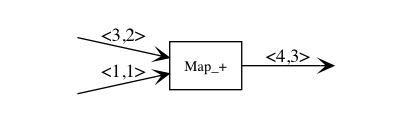
\includegraphics[width=0.6\textwidth]{fig/map.png}
	\end{center}
\end{example}


%the Xducer $\constaf{a}$ outputs the const $a$ until the control stream reaches EOS.
%
%\begin{example} \emph{$\constaf{3}$ with control stream $\c = \<(),()\'>$:}\\
%	\begin{center}
%		
\includegraphics[width=0.6\textwidth]{fig/const3.png}
%	\end{center}
%\end{example}

	

As we have mentioned before, the dataflow of an SVCODE program is basically a DAG, where each Xducer stands for one node. 
The \wc block is only a subgraph that may be added to the DAG at runtime,  
and \sc another that will be unfolded dynamically.

Figure~\ref{fig-svcode-eg1} shows an example program, with its DAG in Figure~\ref{fig-svcode-dag1}. \\

\begin{figure}[H]
	\begin{lstlisting}[style=svcode-style]
	S1 := Const_3();
	S2 := ToFlags(S1);
	S3 := Usum(S2);
	[S4] := WithCtrl(S3,[], 
	          S4 := Const_1();
	        )
	S5 := ScanPlus(S2, S4);
	\end{lstlisting}	
	\caption{A small SVCODE program \label{fig-svcode-eg1}}
\end{figure}
%	S6 := Usum(S2);
%	[S7] := WithCtrl(S6, [S5], 
%	[S7] := SCall(plus1, [S5])
%	)
\hspace{1cm}

\fig{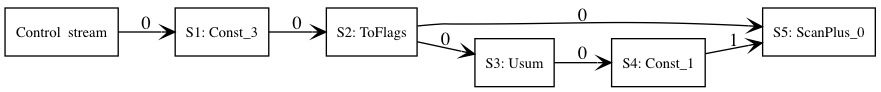
\includegraphics[width=1.1\textwidth]{fig/xducerDag2.png}}{
	Dataflow DAG for the code in Figure~\ref{fig-svcode-eg1} (assuming S3 is nonempty).
	\label{fig-svcode-dag1}
	Note that, for simplicity, the control stream is added as an explicit supplier only to Xducer $\consta{a}$.
}


When we talk about two Xducers $A$ and $B$ connected by an arrow from $A$ to $B$ in the DAG, we call $A$ a $producer$ or a $supplier$ to $B$, and $B$ a $consumer$ or a $client$ of $A$. 
As an Xducer can have multiple suppliers, we distinguish these suppliers by giving each of them an index, called a $channel \ number$. 
In Figure~\ref{fig-svcode-dag1}, the channel number is labeled above each edge. 
For example, the Xducer S2 has two clients, S3 and S5, for both of whom it is the No.0 channel;  Xducer S5 has two suppliers: S2 the No.0 channel and S3 the No.1. 






\section{Translating \mysnesl to SVCODE}
In Section~\ref{sec:valrep}, we have seen the idea of how a high-level value of \mysnesl can be represented as a binary tree of low-level stream values.
At the compiling time, we use a structure $\STree$ (stream id tree) to generalize a binary tree of stream ids, so that the high-level variables and the low-level ones can be connected: 
$$ \STree \ni \st ::= \s \ | \ (\st_1,\st_2) $$
Thus the translation environment $\del$ is a mapping from high-level variables to stream trees:
 $$\del = [x_1 \|-> \st_1,..., x_i \|-> {\st_i}] $$ 

Another important component maintained at the compiling time is a fresh stream id, which has not been used yet. 
It will be assigned to the defined stream(s) of the next generated instruction.

We will use the symbol ``$\Ra$" superscripted with the fresh id to denote the translation relation. 
Also, for clarity, we

\subsection{Expression translation}

A \mysnesl expression will be translated to a pair of an SVCODE program $p$ and a stream tree $\st$ whose stream values representing the high-level evaluation result.

The translation for constants, variables and pairs are straightforward. For example, a pair $(x,4)$ will be translated to an instruction $s_0 := \constaf{4}$ with stream tree $(s,s_0)$, assuming in the context $x$ is bound to $s$ and $s_0$ is a fresh id:   
$$[x \|-> \s] \Env (x,4)  \Ra^{s_0} (s_0 := \constaf{4}, (s,s_0))$$ 

For a let-binding  first adding a new binding to $\del$ and then translating the subexpression in the new environment.

The most interesting case may be the general comprehension.
$\Comp{e_1}{x}{y}{x_1,...,x_j}$, where 



\fig{
 \Jug{\Trans{\del}{e}{\s_0}{\s_1}{\sfun{p}{\st}}}


	\PT{\AC{\Trans{\del}{e_1}{\s_0}{\s_0'}{\sfun{p_1}{\st_1}}}
		\AC{\Trans{\del[x \|-> {\st_1}]}{e_2}{\s_0'}{\s_1}{\sfun {p_2} {\st}}}
		\BC{\Trans{\del}{\Let{x}{e_1}{e_2}}{\s_0}{\s_1}{\sfun {p_1;p_2} {\st}}}
	}\\[3ex]

%TODO: fix and add more 	
	???! TODO:fix
	\PT{
		\AC{\Trans{[x \|-> {\st_1}, \j{x_i \|-> \st_i}]}{e}{\s_0+1+j}{\s_1}{\sfun{p_1}{\st}}}
		\RiLa{\left(
			\begin{aligned}
				\del(y) = &  \ (\st_1,\s_b) \\
				\j{\del(x_i) = & \ \st_i'} \\
				p = & \ \sdef{\s_0}{\usum(\s_b)}; \\
				& \ \j{\sdef{\s_i}{\distrf{\s_b}{\s_i'}};} \\
				& \ \withctrl{\s_0}{p_1}{\Sin}{\Sout} \\
				\Sin = &  \ \FV{p_1} \\
				\Sout = & \ \overline{\st} \cap \dv{p_1} \\
				\s_{i+1} = & \ \s_i + 1, \forall i \in \{0,...,j-1\} \\
			\end{aligned}
			\right)}
		\UC{\Trans{\del}{\Comp{e}{x}{y}{\usevars}}{\s_0}{\s_1}
			{ \sfun{p} {(\st,\s_b)}}}
	}\\[10ex]	
}{Translation rules for \mysnesl expressions \label{fig-trans-snesl1}}
	
% Auxiliary 


\subsection{Built-in function translation}
The function call of a high-level built-in function will be translated to a few lines of SVCODE instuctions.

	\PT{
	\AC{\Transf{\hcall}{\replc{k}{st}}{\s_0}{\s_1}{\sfun{p}{\st}}}
	\RiLa{((\del(x_i)=\st_i)^k_{i=1})}
	\UC{\Trans{\del}{\hcall \Tupk{x}}{\s_0}{\s_1}{\sfun{p}{\st}}}
}\\[5ex]


\fig{
\Jug{\Transf{\hcall}{\replc{k}{st}}{\s_0}{\s_1}{\sfun{p}{\st}}} 
			
	\PT{
		\Axiom{\Transf{\oplus}{\s_1,...,s_k}{\s_0}{\s_0+1}
			\sfun{\sdef{\s_0}{\map{\oplus}(\s_1,...,\s_k)}}{\s_0}}
	}\\[10ex]
	\PT{
		\AC{}
		\RiLa{\left( \begin{aligned}
				\s_{i+1} & = \s_i + 1, \forall i \in \{0,...,3\} \\
				p= & \sdef{\s_0}{\toflag(\s)} ; \\ 
				& \sdef{\s_1}{\usum(s_0)} ; \\
				& \withctrl{\s_1}{\sdef{\s_2}{\consta{1}()}}{[\s_1]}{[\s_2]}; \\
				& \sdef{\s_3}{\scan_{0}(\s_0,s_2)}
			\end{aligned}\right)
		}
		\UC{\Transf{\iotan}{\s}{\s_0}{\s_4}{\sfun{p} {(\s_3,\s_0)}}}
	}\\[4ex]
(will add more)
%TODO add more
}{Translation of built-in functions \label{fig-trans-builtin}}


\subsection{User-defined function translation}
A user-defined function $function \  f(x_1: \tau_1, ..., x_k: \tau_k): \tau = e $ will be translated to an SVCODE function
$([\S_1], p, \ol{\st})$, where $\Trans{[x_1 \|-> st_1,..., x_k \|-> \st_k ]}{e}{0}{s_1}{\sfun{p}{\st}}$ and ...
$$ tp2tree : \tau \ra \STree  $$ 
%TODO 


\section{Eager interpreter}
Recall that an SVCODE program is a list of instructions each of which defines one or more streams. 
The eager interpreter executes the instructions sequentially, assuming the available memory is infinitely large, which is the critical difference between the execution models of the eager and streaming interpreters.

For an eager interpreter, since there is always enough space, a new defined stream can be entirely allocated in memory immediately after its definition instruction is executed.
In this way, traversing the whole program only once will generate the final result, even for recursions.
The streaming model of SVCODE does not show any of its strengths here; the interpreter will perform just like a NESL's low-level interpreter. 


As we will add a limitation to the memory size in the streaming model, it is reasonable to consider the eager version as an extreme case with the largest buffer size of the streaming one. 
In this case, much work can be simplified or even removed, such as the scheduling since there is only one sequential execution round. 
Thus the correctness, as well as the time complexity, is the easiest to analyze, which can be used as a baseline to compare with the streaming version with different buffer sizes.


\subsection{Dataflow}
In the eage model, a Xducer consumes the entire input streams at once and output the entire stream immediately. 
The dataflow DAG is established gradually as Xducers are activated one by one.   
%TODO An example ?

\subsection{Cost model}
The low-level work cost in the eager model is the total number of consumed and produced elements of all Xducers, and the step is merely the number of activated Xducers. 
By activated we mean the executed Xducer definitions, because the stream definitions inside a \wc block may be skipped, in which case we will not account for the steps for those definitions. 


\section{Streaming interpreter}
As we have mentioned before, the execution model of streaming interpreter does not assume an infinite memory; instead, it only uses a limited size of memory as a buffer. 
If the buffer size is relatively small, then most of the streams cannot be materialized entirely at once. 
As a result, the SVCODE program will be traversed multiple times, or there will be more scheduling rounds. 
The dataflow of the streaming execution model is still a DAG, but the difference from the eager one is that each Xducer maintains a small buffer, whose data is updated each round. 
The final result will be collected from all these scheduling rounds.

Since in most cases we will have to execute more rounds, some extra setting-up and overhead seem to be inevitable.
On the other hand, exploiting only a limited buffer increases the efficiency of space usage. 
In particular, for some streamable cases, such as an exclusive scan, the buffer size can be as small as one (and by one we do not mean one bit or byte of physical memory, but rather a conceptual, minimal size).


\subsection{Processes}
In the streaming execution model, the buffer of a Xducer can be written only by the Xducer itself, but can be read by many other Xducers. 
We define two states for a buffer:
And it has two states: 
\begin{itemize}
	\item \filling state : the buffer is not full, and the Xducer is producing or writing data to it; any other trying to read it has to wait, or more precisely, enters a read-block state.

	\item \draining state: the buffer must be full; the readers, including the read-blocked ones, can read it only in this state; if the Xducer itself tries to write the buffer, then it enters a write-block state.
\end{itemize}

The condition of switching from \filling to \draining is simple: when the buffer is fully filled. 
But the other switching direction takes a bit more work to detect: all the readers have read all the data in the buffer. We will come to this later.


A notable special case is when the Xducer produces its last chunk, whose size may be less than the buffer size thus can never turn the buffer to a draining mode.
To deal with this case, we add a flag to the draining state to indicate if it is the last chunk of the stream. 
Thus, the definition of a buffer state is as follows:
$$\bufst = \{\filling \ \a, \ \draining \ \a' \ b \} $$


In addition to maintaining the buffer state, a Xducer also has to remember its suppliers so that it is not necessary to specify the suppliers repeatedly each round. 
Actually, once a dataflow DAG is established, it is only possible to add more subgraphs to it due to an unfolding of a \wc block or a \sc instruction; the other parts uninvolved will be unchanged until the execution is done.


Since Xducers have different data rates (the size of consumed/produced data at each round), it is also important to keep track of the position of the data that has been read, which can be represented by an integer.
Also, it is possible that a Xducer reads from the same supplier multiple times but with different data rates, in which case only a pair of stream id and an integer is not enough to distinguish all the different read cursors. 
Thus we need a third component, the channel number, to record the state of each reader, as we have shown in Figure~\ref{fig-svcode-dag1}.
As a result, we must have a client list $\clis$ of elements of type $(\SId, \int, \int) $

Now we define a structure $process$, a tuple of four components including a Xducer, as the node on the streaming DAG:

$$ \proc  =  (\bufst, \S, \clis, \xducer) $$

where $\S$ is the stream ids of the suppliers. An example process of Xducer $\map{+}$ can be found in Figure~\ref{fig:process}.

\begin{figure}
	\centering
	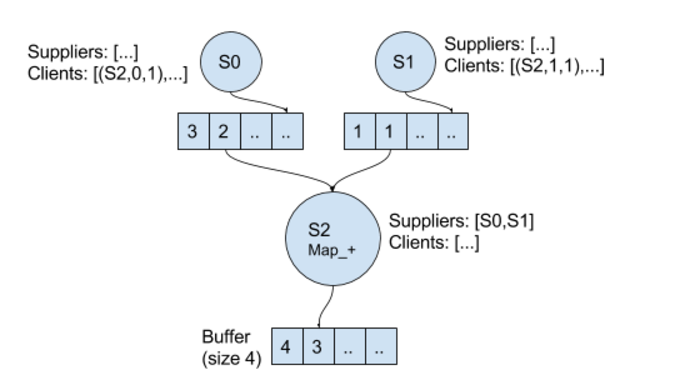
\includegraphics[width=0.9\linewidth]{fig/process}
	\caption{A process S2 of Xducer $\map{+}$. 
		It reads a 2 from S0's buffer and a 1 from S1's buffers, then writes a 3 to its own buffer.}
	\label{fig:process}
\end{figure}

The Xducer inside a process is the action-performing unit. 
We classify the atomic actions of a Xducer into three:
\begin{itemize}
	\item \pin: read one element from one supplier's buffer.
	\item \pout : write one element to its own buffer.
	\item \done: shutdown itself, no read or write any more.
\end{itemize}

In this way, a Xducer's actions can be considered as a sequential list of these three atomics.
For example,  the $\map{+}$ Xducer's action will be repetitions of two \pin s (reads from two suppilers respectively) followed by one \pout, and 
a \done \ action can be added where we want to shut down the Xducer: 
$$[\pin_0, \pin_1, \pout, \pin_0, \pin_1, \pout,... ,\done]$$
 where the subscripts of \pin indicates reading different suppliers.

In our practical implementation, we use a strategy to make the Xducer self-shutdown: we add an extra input stream, the control stream, to each Xducer,
and the Xducer will shut itself down when its read-cursor on the control stream reaches the end, i.e., it reads an EOS (end of stream) from the control stream.


A process is responsible for managing its buffer and Xducer. 
The activity of a process can be described as follows:


 \begin{table}[H]\large
 	\centering
 	\begin{tabular}{|l|p{0.25\columnwidth}|p{0.25\columnwidth}|l|}  
 		\hline
 		 \diagbox{Xducer \\ action}{Buffer \\ state} & \filling & \draining \texttt{F} & \draining \texttt{T} \\ \hline
 		\pin  & Process read  &  Process read  & impossible \\
 		\hline
 		\pout &  write one element to buffer;
 		if buffer is full, switch to \draining \texttt{F}    &    enter write-block     & impossible \\ 
 		\hline
 		\done &  switch to \draining \texttt{T}      & switch to \draining \texttt{T}   & \skip  \\ 
 		\hline
 	\end{tabular}
 \caption{Process actions. }
 \end{table}

Process read:

\begin{itemize}
	\item if the supplier's buffer state is \draining, and the read-cursor shows the process has not yet read all the data, then the process reads one element successfully
	\item if the supplier's buffer state is \draining, but the read-cursor shows the process has read all the data, or the supplier's buffer state is \filling, then the process enters a read-block state
\end{itemize}

full-check: if the buffer is full, switch it to \draining \texttt{F} state.

allread-check: if all the clients have read all the data of the buffer, switch it to \filling state.


\subsection{Scheduling}
The streaming execution model consists of two phases:
\begin{enumerate}[(1)]
\item Initialization \\
In this phase, the interpreter establishes the initial DAG by traversing the SVCODE program. The cases are:
\begin{itemize}
	\item initialize a sole stream definition $\sdef{s}{\lcall(s_1,...,s_k)}$: \\
	This is to set up one process $\s$:
	\begin{itemize}
		\item set its suppilers $\S$ = $[s_1,...,s_k]$
		\item add itself to its suppliers' $\clis$ with the corresponding channel number $\in \{1,...,k\}$ and a read-cursor number 0
		\item empty buffer of state \filling
		\item set up the specific Xducer $\lcall$
	\end{itemize}

	
	\item initialize a function call  $\scall{f}{[s_1,...,s_n]}{[s_1',...,s_m']}$: \\
	A user-defined function at runtime can be considered as another DAG, whose nodes(processes) of the formal arguments are missing. 
	So the interpreter just adds the function's DAG to the main program's DAG 
	and replaces the function's formal arguments with the actual parameters $[s_1,...,s_n]$, and the formal return ones with the actual ones $[s_1',...,s_m']$.  

	
	\item initialize a \wc block $\withctrl{\s_c}{p}{\Sin}{\Sout}$ \\
	At the initialization phase, the interpreter does not unfold $p$; instead, it mainly does the following two tasks:	
	\begin{itemize}
		\item prevents all the import streams of $\Sin$ from producing one more chunk (a full buffer) of data before the interpreter knows whether $s_c$ is an empty stream or not.
		\item initializes all the import streams of $\Sout$ as dummy processes that do not produce any data
	\end{itemize}
	Note that the practical approach for achieving these two goals can be various.
	
\end{itemize}


\item Loop scheduling. \\ 
This phase is a looping procedure. The condition of its end is that all the Xducers have shutdown, and all the buffers are in $\draining \T$ state. 

In a single scheduling round, the processes on the DAG are activated one by one from small to large.
The active process acts as Table~\ref{fig:process} shows, until it enters a read-block or write-block state, or it is skipped.  
The results collected from each round consist entire streams as the final result.

As long as a real (not dummy) process has been set up, it will keep working until its Xducer shutdown. 
The only crucial task in each round is to judge whether to unfold a \wc block or not. The judgment depends on the buffer state of the new control stream.
Note that the new control stream must be some real process
defined earlier than the code inside a \wc block. 

\begin{itemize}
	\item \filling$\emptyv$: the new control process has not produce any data yet, so the judgment cannot be made this round, thus delayed to the next round
	\item \draining$\emptyv \ \T$ : the new control stream is empty, thus no need to unfold the code, just sets the export list streams also empty, and performs some other necessary clean-up job  
	\item other cases: the new control stream must be nonempty, thus the interpreter can unfold the code now
\end{itemize}







	
\end{enumerate}

\subsection{Cost model}
Since we have defined the atomic actions of Xducers, it is now easy to define the low-level cost:
\begin{description}
	\item[Work] = the total number of \pin and \pout \  of all processes
	\item[Step] = the total number of switches from \filling to \draining of all processes
\end{description}


\subsection{Recursion}

In SVOCDE, a recursive function call happens when the function body of $f$ from the instruction $\scall{f}{[s_1,...,s_m]}{[s_1',...,s_n']}$ includes another \sc 
calling  $f$ as well.

As we have shown, for a non-recursive \sc, the effect of interpreting this instruction is almost transparent. 
For a recursive one, there is not much difference except one crucial point: the recursive \sc must be wrapped by a \wc block, otherwise it can never terminate;
at each time of interpreting an inline \sc, the function body is unfolded, but the \wc instruction inside it will stop its further unfolding, that is, the stack-frame number only grows by one. 

At the high level, a well-defined SNESL program should use some conditional to decide when to terminate the recursion. 
As the only conditional of SNESL is the restricted comprehension, which is always translated to a \wc block wrapping the expression body.
Thus we can guarantee that a recursion that can terminate at the high level will also terminate at the low level. 


\begin{example}
\end{example}
\begin{lstlisting}[style=nesl-style]
  -- buffer size 1
  
  -- define a function to compute factorial
  > function fact(x:int):int = if x <= 1 then 1 else x*fact(x-1)
  
  -- running example
  > {{fact(y): y in &x} : x in {5,10}}
  {{1,1,2,6,24},{1,1,2,6,24,120,720,5040,40320,362880}} :: {{int}}
\end{lstlisting}


[?? Optional] The function body of  \texttt{fact}:
%\lstinputlisting[style=svcode-style]{code/fact.svcode}

The translated SVCODE of the expression:
\lstinputlisting[style=svcode-style]{code/fact1.svcode}



\subsection{Deadlock}
An inherent tough issue of the streaming execution model is the risk of deadlock, which is mainly due to the limitation of available memory and the irreversibility (maybe ?) of time.
In general, we classify deadlock situations into two types: soft deadlock, which can be detected and broken relatively easily but not necessarily by enlarging the buffer size, and hard deadlock, which can only be solved by enlarging the buffer size. 

\begin{itemize}

\item Soft deadlock: \\

One case of soft deadlock can be caused by trying to traverse the same sequence multiple times. 
A simpler example:

\begin{example} \emph{A soft deadlock caused by travesing the sequence $x$ two times.} \label{eg:deadlock1}
\end{example}
	\begin{lstlisting}[style=nesl-style]
  > let x = {1} in x ++ x
  Deadlock!
\end{lstlisting}

There are at least two feasible solutions to this case.
One is manually rewriting the code to define new variables for the same sequence, as the following code shows :\\

\begin{lstlisting}[style=nesl-style]
  > let x = {1}; y = {1} in x ++ y
  {1,1} :: {int}
\end{lstlisting}

%Or, for the full SNESL supporting vectors, the 

The other can be done by optimizing the compiler to support multi-traversing check and automatic 
redefinition of retraversed sequences. 
As the code grows more complicated, locating the problem can become much harder, thus a smarter compiler is definitely necessary, which is worth some future investigation.\\


Another case of soft deadlock can be due to the different data rates of processes, which leads to a situation where some buffer(s) of $\filling$ state can never turn to \draining. 
For example, the following expression tries to negate the elements that can be divided by 5 exactly of a sequence.
\begin{example}\emph{ A soft deadlock that can be broken by stealing}
\end{example}
\begin{lstlisting}[style=nesl-style]
  -- buffer size 4 
 > concat({{-x | x % 5 == 0} ++ {x | x %5 != 0} :  x in &10})
 {0,1,2,3,4,-5,6,7,8,9} :: {int}
\end{lstlisting}

In this example, the sequence contains elements from 0 to 9; the subsequence of the negated numbers, which only contains 0 and -5, are concatenated with the one of the other eight numbers. Since these two subsequences are generated at different rates, 
If we minimize the buffer size to 1, then the deadlock can be broken since buffer of size one can always turn to \draining mode as long as there is one element generated. 
In our implementation, we use an automatic solution for this case, called $stealing$. 
The idea is that when a deadlock is detected, we will first switch the smallest process with a \filling buffer, into \draining mode, to see if the deadlock can be broken; if not, we repeat this switch until the deadlock is broken; otherwise, it may be a hard deadlock.

Since the stealing strategy is basically a premature
switch from \filling to \draining, the low-level step cost is possible to be affected. More precisely,  it can be increased by a certain amount, which depends on the concrete program and the buffer size. 
The effect of stealing on the cost model can also be investigated as future work.


\item Hard deadlock: \\

This type of deadlock is mainly because of insufficient space.

\begin{example} \emph{The following SNESL function {\ttfamily oeadd} risks a hard deadlock. Given an integer sequence with an equal number of odd and even numbers, this function will try to perform addition on a pair of an odd and an even number with the same index from their respective subsequences.} 
\end{example}

\lstinputlisting[style=nesl-style]{code/harddeadlock.snesl} 
\hspace{0.3cm}

If we give a proper argument, for example, an sequence of odds and evens interleaving with each other(??? not clear), it may never deadlock, even with a buffer of size one. 
But if there is a relatively large distance between any odd-even pair, the code will deadlock.  \\
  
\begin{lstlisting}[style=nesl-style]
-- buffer size 1

> oeadd(&30)
{1,5,9,13,17,21,25,29,33,37,41,45,49,53,57} :: {int}

> oeadd({1,3,5,7,0,2,4,8})
Deadlock!
\end{lstlisting}


This type of deadlock can only be broken by enlarging the buffer size. 


\end{itemize}


\subsection{[optional] Evaluation}
Some possibilies for improving the scheduling:

\begin{itemize}
\item The processes in a block state will be activated in the next scheduling round, but it may still  block itself immediately since the blocking condition still holds. So a better strategy can be 

\item The processes are activated only one by one, even though some of them can be data-independent, this simulates a SIMD machine execution. But it should be able to be optmized to support MIMD machine. 
Evaluation of some high-level expressions, such as the evaluation of the components of a tuple or a function call , can be executed in parallel as well.


\end{itemize}

\subsection{[optional] Examples}

\lstinputlisting[style=nesl-style]{code/uc_scanred.snesl}


%\section{Translation}

\subsection{Translation rules}
\begin{enumerate}[(1)]
	\item Stream tree: $$ \STree \ni \st ::= \s \ | \ (\st_1,\s) $$
	\item Convert a stream tree to a list of  stream ids:
	\begin{align*}
	&\bar{}: \STree \-> \S \\
	&\overline{\s} = [s] \\
	&\overline{(\st,s)} = \overline{st} {\++} [s]
	\end{align*}
	
	
	\item Translation environment: $$\del = [x_1 \|-> \st_1,..., x_i \|-> {\st_i}] $$ 
	
	
\end{enumerate}

\begin{itemize}	
	
	\item \Jug{\Trans{\del}{e}{\s_0}{\s_1}{\sfun{p}{\st}}}
	
	\PT{\AC{}
		\RiLa{(\del(x)= \st)}
		\UC{\Trans{\del}{x}{\s_0}{\s_0}{\sfun{\epsilon}{\st}}}
	}
	\PT{\AC{\Trans{\del}{e_1}{\s_0}{\s_0'}{\sfun{p_1}{\st_1}}}
		\AC{\Trans{\del[x \|-> {\st_1}]}{e_2}{\s_0'}{\s_1}{\sfun {p_2} {\st}}}
		\BC{\Trans{\del}{\Let{x}{e_1}{e_2}}{\s_0}{\s_1}{\sfun {p_1;p_2} {\st}}}
	}
	
	\PT{
		\AC{\Transf{\hcall}{\replc{k}{st}}{\s_0}{\s_1}{\sfun{p}{\st}}}
		\RiLa{((\del(x_i)=\st_i)^k_{i=1})}
		\UC{\Trans{\del}{\hcall \Tupk{x}}{\s_0}{\s_1}{\sfun{p}{\st}}}
	}\\[5ex]
	
	\PT{
		\AC{\Trans{[x \|-> {\st_1}, \j{x_i \|-> s_i}]}{e}{\s_0+1+j}{\s_1}{\sfun{p_1}{\st}}}
		\RiLa{\left(
			\begin{aligned}
				\del(y) = &  \ (\st_1,\s_b) \\
				\j{\del(x_i) = & \ \s_i'} \\
				p = & \ \sdef{\s_0}{\usum(\s_b)}; \\
				& \ \j{\sdef{\s_i}{\distrf{\s_b}{\s_i'}};} \\
				& \ \withctrl{\s_0}{p_1}{\Sin}{\Sout} \\
				\Sin = &  \ \FV{p_1} \\
				\Sout = & \ \overline{\st} \cap \dv{p_1} \\
				\s_{i+1} = & \ \s_i + 1, \forall i \in \{0,...,j-1\} \\
			\end{aligned}
			\right)}
		\UC{\Trans{\del}{\Comp{e}{x}{y}{\usevars}}{\s_0}{\s_1}
			{ \sfun{p} {(\st,\s_b)}}}
	}
	
	\vspace{2cm}
	
	\item Auxiliary \Jug{\Transf{\hcall}{\replc{k}{st}}{\s_0}{\s_1}{\sfun{p}{\st}}}
	
	\PT{
		\Axiom{\Transf{\constn{n}}{}{\s_0}{\s_0+1}
			\sfun{\sdef{\s_0}{\consta{n}()}}{\s_0}  }
	} \\ [6ex]
	
	\PT{
		\AC{}
		\RiLa{\left( \begin{aligned}
				\s_{i+1} & = \s_i + 1, \forall i \in \{0,...,3\} \\
				p= & \sdef{\s_0}{\toflag(\s)} ; \\ 
				& \sdef{\s_1}{\usum(s_0)} ; \\
				& \withctrl{\s_1}{\sdef{\s_2}{\consta{1}()}}{[\s_1]}{\overline{\s_2}}; \\
				& \sdef{\s_3}{\scan_{0}(\s_0,s_2)}
			\end{aligned}\right)
		}
		\UC{\Transf{\iotan}{\s}{\s_0}{\s_4}{\sfun{p} {(\s_3,\s_0)}}}
	}\\[4ex]
	
	\PT{
		\Axiom{\Transf{\plusn}{\s_1,\s_2}{\s_0}{\s_0+1}
			\sfun{\sdef{\s_0}{\maptwo{+}(\s_1,\s_2)}}{\s_0}}
	}
	
\end{itemize}


\subsection{Value representation}
\begin{enumerate}
	\item SVCODE values: $$\SvVal \ni \v ::= \a \ | \ (\v,\b) $$
	\item SVCODE values concatenation: \\ 
	\begin{align*}
	&\++: \SvVal \->  \SvVal \-> \SvVal \\
	&\vapp{\<\a_1,...,\a_i\'>}{\<\a_1',...,\a_j'\'>} = \<\a_1,...,\a_i,\a_1',...,\a_j'\'> \\
	&\vapp{(\v_1,\b_1)}{(\v_2,\b_2)} = (\vapp{\v_1}{\v_2}, \vapp{\b_1}{\b_2})
	\end{align*}
	
	\item SVCODE value construction from a stream tree: \\
	\begin{align*}
	&\sgm : \STree \-> \SvVal \\
	&\sgm(\s) = \a \\
	&\sgm((\st,\s)) = (\sgm(\st), \sgm(\s)) 
	\end{align*}
	
	
	\item Value representation rules
	\begin{itemize}
		
		\item \Jug{\ValRep{v}{\tau}{\v}}
		
		\PT{
			\Axiom{\ValRep{n}{\int}{\singl{n}}}
		}
		\PT{
			\AC{(\ValRep{v_i}{\tau}{\v_i})^k_{i=1}}
			\RiLa{(\v = \v_1 {\++} ... {\++} \v_k)}
			\UC{\ValRep{\Seqk{v}}{\tseq{\tau}}{(\v,\langle \F_1,..., \F_k, \T \rangle)}}
		}
	\end{itemize}
\end{enumerate}




\begin{comment}
\PT{
\AC{\ValRep {\lrange{v_1}{v_k}} {\tau} {\v}}
\UC{\ValRep {\Seqk{v}}{\tseq{\tau}}{(\v,\langle \F_1,..., \F_k, \T \rangle)}}
}\\[4ex]

\item \Jug{\ValRep{\lrange{v_1}{v_k}}{\tau}{\v}}
\PT{
\Axiom{\ValRep{\lrange{n_1}{n_k}}{\int}{\vrange{n_1}{n_k}}}
}
\PT{
\AC{\ValRep{v_i}{\tau}{\v}}
\UC{\ValRep{\lrange{v_1}{v_k}}{\tseq{\tau}}{}}
}

\end{comment}



\begin{lem}[\textbf{Value translation backwards determinism}]
	If $\ValRep{v}{\tau}{w}$, $\ValRep{v'}{\tau}{w}$,
	then $v=v'$.
\end{lem}



\section{Correctness proof}

\subsection{Definitions}
We first define a binary relation $\~\S$ on stores to denote that two stores are $similar$: they have identical domains, and their bound values by $\S$ are the same. 
We call this $\S$ an $overlap$ of these two stores.

\begin{defi}[\textbf{Stores similarity}]
	\label{def-sgm-sim}
	
	$\sgm_1 {\~{\S}} \sgm_2 $
	iff \\
	(1) $dom(\sgm_1) = dom(\sgm_2)$ \\
	(2) $\forall s \in \S.\sgm_1(s)= \sgm_2(s)$ \\
\end{defi}

According to this definition, it is only meaningful to have $\S  \subseteq dom(\sgm_1)$ (= $dom(\sgm_2)$).  
When $\S = dom(\sgm_1) = dom(\sgm_2)$, $\sgm_1$ and $\sgm_2$ are identical. 
It is easy to show that this relation $\overset{\S}{\sim}$ is symmetric and transitive.
\begin{itemize}
	\item If $\sgm_1 \~\S \sgm_2$, then $\sgm_2 \~\S \sgm_1$.
	\item If $\sgm_1 \~\S \sgm_2$ and $\sgm_2 \~\S \sgm_3$, then $\sgm_1 \~\S \sgm_3$.
\end{itemize}


We also define a binary operation $\x\S$ on stores to denote a kind of specical concatenation of two similar stores: 
the $concatenation$ of two similar stores is a new store, in which the bound values by $\S$ are from any of the parameter stores, and 
the others are the concatenation of the values from the two stores. 
In other words, a $concatenation$ of two similar stores is only a concatenation of the bound values that $maybe$ different in these stores.
\begin{defi}[\textbf{Store Concatenation}] \label{def-sgm-join}
	For $\sgm_1 \~\S \sgm_2$,
	$\sgm_1 \x{\S} \sgm_2 = \sgm$ where \\
	$\sgm(s) =
	\begin{cases}
	\sgm_1(s) (=\sgm_2(s)), & s \in \S\\
	\sgm_1(\s) {\++} \sgm_2(s), & s \notin \S \\
	\end{cases} $
\end{defi}

\begin{lem} \label{lem-join1}
	If $\sgm_1 \x{\S} \sgm_2 = \sgm$, 
	then $\sgm_1 \~{\S} \sgm$ and $\sgm_2 \~{\S} \sgm.$
\end{lem}
This lemma says that the concatenation result of two similar stores is still similar to each of them.
%\begin{proof}
%	According to Definition \ref{def-sgm-join}, it is clear that $dom(\sgm) = dom(\sgm_1)$, and $\forall s \in \S. \sgm(s) = \sgm_1(s)$. Then by Definiton \ref{def-sgm-sim}, $\sgm \~\S \sgm_1$
%\end{proof}


\begin{lem} \label{lem-psi-join}
	If \begin{enumerate}[(i)]
	 \item $\sevalfg{\lcall}{\a_{1},...,\a_{k}}{\c_1}{\a_0}$ by some derivation $\MP_1$
	 \item $\sevalfg{\lcall}{\a'_{1},...,\a'_{k}}{\c_2}{\a_0'}$ by some $\MP_2$,
	\end{enumerate}
	then $\sevalfg{\lcall}{\a_{1} {\++} \a'_{1},...,\a_{k} {\++} \a'_{k}}{\c {\++} \c'}{\a {\++} \a'}$ by some $\MP_3$.
\end{lem}

\begin{proof}
\def\cc{\c_1 {\++} \c_2}
\def\aap#1{\a_{#1} {\++} \a_{#1}'}
\def\zk#1{(#1)^k_{i=0}}

	There are two possibilities: 
	\begin{itemize}
		\item Case $\MP_1$ uses $\PName{X-Termi}$.\\
		We must have $\zk{\a_i=\emptyv}$ and $\c_1 = \emptyv$.
		Then $\zk{\aap{i} = \a_i'}$, and $\cc = \c_2 $. Take $\MP_3
		= \MP_2$ and we are done. \\
		
		\item Case $\MP_1$ uses $\PName{X-Loop}$. \\
	   Assume $\c_1 = \<() | \c_1' \'>$, then we have 
		$$
		\PT{
			\UCN{\MP_{11}}{\block{\a_{11}}{\a_{k1}}{\a_{01}}}
			\UCN{\MP_{12}}{\sevalf{\a_{12}}{\a_{k2}}{\c_1'}{\a_{02}}}
 			\LeLa{\MP_1 = }
			\BC{\sevalf{\a_1}{\a_k}{\< c_0 | \c_1' \'>}{\a_0}}
		}$$
	    with $\zk{\a_i = \vapp{\a_{i1}}{\a_{i2}}}$.\\
	    
	    By IH on $\MP_{12}$ with $\MP_2$, we get a derivation $\MP_4$ of 
	    $$\sevalfg{\lcall}{\a_{12} {\++} \a_1',...,\a_{k2} {\++} \a_k'}{\c_1' {\++} \c_2 }{\a_{02} {\++} \a_0'}$$
	    
	    Then using the rule $\PName{X-Loop}$ we can build a derivation $\MP_5$ as follows:
	    	$$
	    \PT{
	    	\UCN{\MP_{11}}{\block{\a_{11}}{\a_{k1}}{\a_{01}}}
	    	\UCN{\MP_{4}}{\sevalfg{\lcall}{\a_{12} {\++} \a_1',...,\a_{k2} {\++} \a_k'}{\c_1' {\++} \c_2 }{\a_{02} {\++} \a_0'}}
	    	\BC{\sevalf{\a_{11} {\++} {(\a_{12} {\++} \a_1')}}
	    		        {\a_{k1} {\++} {(\a_{k2} {\++} \a_k')}}
	    		        {\< () | \c_1' {\++} \c_2 \'>}
	    		        {\a_{01} {\++} {(\a_{02} {\++} \a_0')}}}
	    }$$
	    Since it is clear that 
	    $$\forall i \in \{0,...,k\}. \ \a_{i1} {\++} (\a_{i2} {\++} \a_i') = (\a_{i1} {\++} \a_{i2}) {\++} \a_i' = \a_i {\++} \a_i' $$
	    $$ \< () | \c_1' {\++} \c_2 \'> = \< () | \c_1' \'> {\++} \c_2 = \c_1 {\++} \c_2 $$
	    so take $\MP_3 = \MP_5$ and we are done. 
	    
	\end{itemize}
	
\end{proof}

\begin{lem} \label{lem-emp-join}
	If 
	\begin{enumerate} [(i)]
		\item $\sgm_1 \~{S} \sgm_2$
		\item $\seval{p}{\sgm_1}{\c}{\sgm}$
		\item $\FV{p} \cap \S = \emptyset$
		\item $\forall s \in \FV{p}. \sgm_2(s) = \emptyv$
	\end{enumerate}
	then 
	\begin{enumerate}[(i)]
		\setcounter{enumi}{4}
		\item $\seval{p}{\sgm_1 \x{\S} \sgm_2}{\c}{\sgm'}$
		\item $\forall s' \in \dv{p}. \sgm(s') = \sgm'(s')$
	\end{enumerate}
\end{lem}

\begin{lem} \label{lem-emp-join-sym}
	If 
	\begin{enumerate} [(i)]
		\item $\sgm_1 \~{S} \sgm_2$
		\item $\seval{p}{\sgm_2}{\c}{\sgm}$
		\item $\FV{p} \cap \S = \emptyset$
		\item $\forall s \in \FV{p}. \sgm_1(s) = \emptyv$
	\end{enumerate}
	then 
	\begin{enumerate}[(i)]
		\setcounter{enumi}{4}
		\item $\seval{p}{\sgm_1 \x{\S} \sgm_2}{\c}{\sgm'}$
		\item $\forall s' \in \dv{p}. \sgm(s') = \sgm'(s')$
	\end{enumerate}
\end{lem}

\begin{lem} [\textbf{Stores concatenation lemma}] \label{lem-sgm-join}
	If 
	\begin{enumerate}[(i)]
		\item $\sgm_1 \~{\S} \sgm_2$
		\item $\seval{p}{\sgm_1}{\c_1}{\sgm_1'}$ (by some derivation $\MP_1$)
		\item $	\seval{p}{\sgm_2} {\c_2} {\sgm_2'}$ (by some derivation $\MP_2$)
		\item $\FV{p} \cap \S = \emptyset $
	\end{enumerate}
	then $\seval{p}{\sgm_1 \x\S \sgm_2}{\c_1 {\++} \c_2}{ \sgm_1' \x\S \sgm_2' }$ (by $\MP$).
\end{lem}

We need this lemma to prove that the results of single computations inside a comprehension body (i.e. $p$ in the lemma) can be concatenated to express a parallel computation. From the other direction, we can consider this process as distributing or splitting the compuation $p$ on even smaller degree of parallel computations, in which all the supplier streams, i.e., $\FV{p}$, are splitted to
feed the transducers. The splitted parallel degrees are specified by the
control streams, i.e., $\c_1$ and $\c_2$ in the lemma. Other untouched $\SId$s in all $\sgm$s (i.e., $\S$) have no change throughout the process.\\

\begin{proof}
	By induction on the syntax of $p$.
\def\sgmx{\sgm_1 \x{\S} \sgm_2}
\def\sgmpx{\sgm_1' \x{\S} \sgm_2'}
\def\cc{\c_1 {\++} \c_2}

 
	\begin{itemize}
	\item Case $p = \epsilon$. \\
	$\MP_1$ must be $\overline{\seval{\epsilon}{\sgm_1}{\c_1}{\sgm_1}}$, and
	$\MP_2$ must be $\overline{\seval{\epsilon}{\sgm_2}{\c_2}{\sgm_2}}$. \\
	So $\sgm_1' = \sgm_1$, and $\sgm_2' = \sgm_2$, thus $\sgm_1' \x{\S} \sgm_2' = \sgm_1 \x{\S} \sgm_2$. \\
	
	By $\PName{Empty}$, we take $\MP$ = $\overline{\seval{\epsilon}{\sgmx}{\c_1 {\++} \c_2}{\sgmx}}$ and we are done. 
	
\item Case $p = \sdef{\s_l}{\lcall(s_1,...,s_k)}.$ \\
\def\casetwo{\sdef{\s_l}{\lcall\Tupk\s}}	
\def\eqnumtwo#1{eq-lem24-c2-{#1}}
	$\MP_1$ must look like 
	$$\PT{\UCN{\MP'_{1}}{\sevalf{\a_1}{\a_k}{\c_1}{\a}}
			\UC{\seval{\sdef{\s_l}{\lcall\Tupk\s}}{\sgm_1}{\c_1}{\sgm_1[\s_l \|-> \a]}}
	} $$

	and we have 
	    \eq{eq-lem24-c2-1}{(\sgm_1(\s_i) = \a_i)^k_{i=1}}
	
	
    Similarly, $\MP_2$ must look like 
	$$\PT{\UCN{\MP'_{2}}{\sevalf{\a_1'}{\a_k'}{\c_2}{\a'}}
		\UC{\seval{\sdef{\s_l}{\lcall\Tupk\s}}{\sgm_2}{\c_2}{\sgm_2[\s_l \|-> \a']}}
	} $$
	
	and we have
	\eq{eq-lem24-c2-2}{(\sgm_2(\s_i) = \a_i')^k_{i=1}}
	
	So  $\sgm_1' = \sgm_1[\s_l \|-> \a], \sgm_2' = \sgm_2[\s_l \|-> \a']$. \\
	
	From assumption $(iv)$ we have $\FV{\casetwo} \cap \S = \emptyset$,
    that is, 
	\eq{eq-lem24-c2-3}{\{s_1,...,s_k\} \cap \S = \emptyset}

    
    By Lemma \ref{lem-psi-join} on $\MP'_{1}$, $\MP'_{2}$, we get a derivation $\MP'$ of 
    \[ \sevalfg{\lcall}{\a_1  {\++} \a_1',...,\a_k {\++} \a_k' } 
             {\c_1 {\++} \c_2} {\a {\++} \a'} \]
    
    Since $\sgm_1 \~{\S} \sgm_2$, 
    with \eqref{eq-lem24-c2-1},\eqref{eq-lem24-c2-2} and \eqref{eq-lem24-c2-3}, 
    by Definition $\ref{def-sgm-join}$ we have
    \eq{\eqnumtwo{5}}{
	    \forall i \in \{1,...,k\}.\sgmx(\s_i) = \sgm_1(\s_i) {\++} \sgm_2(\s_i) = \a_i {\++} \a_i'}
 	Also, it is easy to prove that $\sgm_1[\s_l \|-> \a] \x{\S} \sgm_2[\s_l \|-> \a'] \~\S \sgmx[\s_l \|-> \a {\++} \a'] $ and \eq{\eqnumtwo{4}}{
 		\sgm_1[\s_l \|-> \a] \x{\S} \sgm_2[\s_l \|-> \a'] = 
 		\sgmx[\s_l \|-> \a {\++} \a']
 	}
 
    Using the rule $\PName{Xducer}$ with $\eqref{\eqnumtwo{5}}$, we can build $\MP''$ as follows
   	$$\PT{\UCN{\MP'}{\sevalfg{\lcall}{\a_1  {\++} \a_1',...,\a_k {\++} \a_k' } 
   			{\c_1 {\++} \c_2} {\a {\++} \a'}}
    	\UC{\seval{\casetwo}{\sgmx}{\c_1 {\++} \c_2}{\sgmx[\s_l \|-> \a {\++} \a']}}
    } $$
   
   
    Replacing $\sgmx[\s_l \|-> \a {\++} \a']$ in $\MP''$ with the left-hand side of $\eqref{\eqnumtwo{4}}$ gives us $\MP$ 
   	$$\PT{\UCN{\MP'}{\sevalfg{\lcall}{\a_1  {\++} \a_1',...,\a_k {\++} \a_k' } 
   			{\c_1 {\++} \c_2} {\a {\++} \a'}}
   		\UC{\seval{\casetwo}{\sgmx}{\c_1 {\++} \c_2}{\sgm_1[\s_l \|-> \a] \x{\S} \sgm_2[\s_l \|-> \a']}}
   	} $$ as required.
   	

\item Case $p = \withctrl{\s_c}{p_0}{\Sin}{\Sout}$ where  
\def\eqnumthree#1{eq-lem24-c3-{#1}}

 \eq{eq-lem24-c3-1}{\FV{p_0} \subseteq \Sin}
 \eq {eq-lem24-c3-2}{\Sout \subseteq \dv{p_0}}

\def\casethree{\withctrl{\s_c}{p_0}{\Sin}{\Sout}}

	From the assumption ($iv$), we have 
	\begin{align*}
	\FV{\casethree} \cap \S & = \emptyset \\
	(\{\s_c\} \cup \Sin) \cap \S & = \emptyset \tag{by definition of $\FV{}$} 
	\end{align*}
	thus 
	\eq{eq-lem24-c3-3}{\{\s_c\} \cap \S = \emptyset}
	\eq{eq-lem24-c3-4}{\Sin \cap \S = \emptyset}
	
    Since \eqref{eq-lem24-c3-1} with \eqref{eq-lem24-c3-4}, we also have 
    	\eq{eq-lem24-c3-6}{\FV{p_0} \cap \S = \emptyset}
    
    Assume $\Sout = [s_1,...,s_j]$. \\	
    There are four possibilities: 
   
    \begin{itemize}


    	\item Subcase both $\MP_1$ and $\MP_2$ use $\PName{Wc-Emp}$. \\
    	
    	So $\MP_1$ must look like 
    	
    	$$\PT{
    		\Axiom{\seval{\casethree}{\sgm_1}{\c_1}{\sgm_1[\s_1 \|-> \emptyv, ..., \s_j \|-> \emptyv]}}
    	}$$
    	and we have   \eq{eq-lem24-c3-5}{  	
    		\forall s \in \{\s_c\} \cup \Sin. \sgm_1(s) = \emptyv}
        thus
    		\eq{eq-lem24-c3-7}{\sgm_1(s_c) = \emptyv}
    	  	\eq{\eqnumthree{8}}{\forall s \in \FV{p_0}. \sgm_1(s) = \emptyv}
    	
    	Similarly,$\MP_2$ must look like  	
    	$$\PT{
    		\Axiom{\seval{\casethree}{\sgm_2}{\c_2}{\sgm_2[\s_1 \|-> \emptyv, ..., \s_j \|-> \emptyv]}}
    	}$$
    	and we have   \eq{eq-lem24-c3-9}{  	
    		\forall s \in \{\s_c\} \cup \Sin. \sgm_2(s) = \emptyv}
    	thus
    	\eq{eq-lem24-c3-10}{\sgm_2(s_c) = \emptyv}
    	\eq{\eqnumthree{11}}{\forall s \in \FV{p_0}. \sgm_2(s) = \emptyv}

 \def\sgmbe#1{\sgm_#1[\j{\s_i \|-> \emptyv}]}
    	
    	So $\sgm_1' = \sgmbe{1}$, $\sgm_2' = \sgmbe{2}$. \\
    	
 	Since $\sgm_1 \~{\S} \sgm_2$, by Definition $\ref{def-sgm-join}$ with \eqref{eq-lem24-c3-3}, \eqref{eq-lem24-c3-4}, and  \eqref{eq-lem24-c3-5}, \eqref{eq-lem24-c3-9}, we have    		
   		\eq{\eqnumthree{8}}{\forall s \in \{\s_c\} \cup \Sin. \sgmx(\s) = \sgm_1(\s) {\++} \sgm_2(s) =  \emptyv}
   		
   		Also, it is easy to show that $\sgmbe1 \~{\S} \sgmbe2$ and 
   		\eq{\eqnumthree{7}}{
   			\sgmbe1 \x{\S} \sgmbe2 = \sgmx[\j{\s_i \|-> \emptyv}]
   		}
   	
    Using $\PName{Wc-Emp}$ with $\eqref{\eqnumthree{8}}$, we build $\MP'$ as follows
   		$$\PT{
   			\Axiom{\seval{\casethree}{\sgmx}{\cc}{(\sgmx)[\j{\s_i \|-> \emptyv}]}}
   		}$$
   	
   	Then replcaing $\sgmx[\j{\s_i \|-> \emptyv}]$ in $\MP'$ with the left-hand side of $\eqref{\eqnumthree{7}}$ gives us $\MP$ of \\
   \makebox[0.9\textwidth][c]{		$$\PT{
   			\Axiom{\seval{\casethree}{\sgmx}{\cc}{\sgmbe1 \x{\S} \sgmbe2}}
   		}$$}
   		as required. \\
   
   	\item Subcase $\MP_1$ uses  $\PName{Wc-Nomemp}$, $\MP_2$ uses $\PName{Wc-Emp}$. \\
  \def\sgmbpp#1{\sgm_{#1}[\j{\s_i \|-> \sgm_{#1}''(\s_i)}]}   	
   	$\MP_1$ must look like
   	$$\PT{
   			\UCN{\MP_1'}{\seval{p_0}{\sgm_1}{\c_1'}{\sgm_1''}}
   			\UC{\seval{\casethree}{\sgm_1}{\c_1}{\sgmbpp1}}
   	}$$
    and we have 
    \eq{\eqnumthree{20}}{\sgm_1(\s_c)= \c_1' = \< () | ...\'>}
   	
   	$\MP_2$ must look like	
   	$$\PT{
   		\Axiom{\seval{\casethree}{\sgm_2}{\c_2}{\sgmbe{2}}}
   	}$$
   	and we have  
   	$\forall s \in \{\s_c\} \cup \Sin. \sgm_2(s) = \emptyv$
   thus
	\eq{\eqnumthree{21}}{\sgm_2(s_c) = \emptyv}
	\eq{\eqnumthree{22}}{\forall s \in \FV{p_0}. \sgm_2(s) = \emptyv}   	
 


	
	So $\sgm_1' = \sgmbpp{1}$, $\sgm_2' = \sgmbe{2}$.

    By Lemma \ref{lem-emp-join} on $\sgm_1 \~{\S} \sgm_2$ with $\MP_1'$, \eqref{\eqnumthree{22}}, \eqref{eq-lem24-c3-6}, we obtain a derivation $\MP_0$
    of 
    $$\seval{p_0}{\sgmx}{\c_1'}{\sgm_0}$$ for some $\sgm_0$, and 
    $$\forall s \in dv(p_0). \sgm_0(s) = \sgm_1''(s), $$
    thus,  with \eqref{eq-lem24-c3-2}, we have
    \eq{\eqnumthree{25}} {(\sgm_0(s_i) = \sgm_1''(s_i))^j_{i=1}}
    

%   		
   	Since $\sgm_1 \~\S \sgm_2$,	by Definition \ref{def-sgm-join} with $\eqref{\eqnumthree{20}}$, $\eqref{\eqnumthree{21}}$, we have \eq{\eqnumthree{27}}{
   		\sgmx(s_c) = \sgm_1(s_c) {\++} \sgm_2(s_c) = \c_1' =  \<()| ...\'>}
   	
   	and it is also easy to prove $\sgmbpp{1} \~\S \sgmbe{2}$ and \eq{\eqnumthree{26}}{
   		\sgmbpp{1} \x{\S} \sgmbe{2} =  
   		 \sgmx[\j{\s_i \|-> \sgm_{1}''(\s_1)}]
   	}	
   
     Using the rule $\PName{Wc-Nonemp}$ with $\eqref{\eqnumthree{27}}$ we can build a derivation $\MP'$ as follows 	
  		$$\PT{
  			\UCN{\MP_0}{\seval{p_0}{\sgmx}{\c_1'}{\sgm_0}}
  			\UC{\seval{\casethree}{\sgmx}{\cc}{(\sgmx) [\j{\s_i \|-> \sgm_0(\s_i)}]}}
  		}$$ 
  	
  	With $\eqref{\eqnumthree{25}}$, we replace $\sgm_0(s_i)$ with $\sgm_1''(s_i)$ for $ \forall i \in \{1,...,j\}$ in $\MP'$, obtaining  
  		$$\PT{
  		\UCN{\MP_0}{\seval{p_0}{\sgmx}{\c_1'}{\sgm_0}}
  		\UC{\seval{\casethree}{\sgmx}{\cc}{(\sgmx) [\j{\s_i \|-> \sgm_1''(\s_i)}]}}
  	}$$ 
  		
  	Then replacing $(\sgmx) [\j{\s_i \|-> \sgm_1''(\s_i)}]$ in $\MP'$ with the left-hand side of $\eqref{\eqnumthree{26}}$, we get $\MP$ of \\
  	 \makebox[0.9\textwidth][c]{\PT{
  	 	\UCN{\MP_0}{\seval{p_0}{\sgmx}{\c_1'}{\sgm_0}}
  	 	\UC{\seval{\casethree}{\sgmx}{\cc}{\sgmbpp{1} \x{\S} \sgmbe{2}}}
  	 }}
    as required. \\
  
	\item Subcase $\MP_1$ uses  $\PName{Wc-Emp}$ and $\MP_2$ uses $\PName{Wc-Nonemp}$. \\	
	This subcase is symmetric to the second one, so the proof is analogous except that this subcase uses Lemma $\ref{lem-emp-join-sym}$ rather than  Lemma $\ref{lem-emp-join}$.\\
 		
	\item Subcase both $\MP_1$ and $\MP_2$ use $\PName{Wc-Nonemp}$. \\
 	$\MP_1$ must look like
 	$$\PT{
 		\UCN{\MP_1'}{\seval{p_0}{\sgm_1}{\c_1'}{\sgm_1''}}
 		\UC{\seval{\casethree}{\sgm_1}{\c_1}{\sgmbpp1}}
 	}$$
 	and 
 	\eq{\eqnumthree{30}}{\sgm_1(\s_c)= \c_1' = \< () | ...\'>}
 	
 	Similarly, $\MP_2$ must look like
 	$$\PT{
 		\UCN{\MP_2'}{\seval{p_0}{\sgm_2}{\c_2'}{\sgm_2''}}
 		\UC{\seval{\casethree}{\sgm_2}{\c_2}{\sgmbpp2}}
 	}$$
 	and 
 	\eq{\eqnumthree{31}}{\sgm_2(\s_c)= \c_2' = \< () | ...\'>}
    
    So $\sgm_1' = \sgmbpp{1}, \sgm_2' = \sgmbpp{2}.$
    
    By IH on $\MP_1'$, $\MP_2'$ with \eqref{eq-lem24-c3-6}, we get a derivation $\MP_0$ of 
    $$\seval{p_0}{\sgmx}{\c_1' {\++} \c_2'}{\sgm_1'' \x{\S} \sgm_2''}$$
    
    Since $ \forall i \in \{1,...,j\}. s_i \notin \S$ ,
    then by Definition $\ref{def-sgm-join}$, we know
    \eq{\eqnumthree{32}}{\sgm_1'' \x{\S} \sgm_2''(\s_i) = \sgm_1''(\s_i) {\++} \sgm_2''(\s_i)}
    
    Also, it is easy to show that $\sgmbpp{1} \~{\S} \sgmbpp{2}$,
    and
   \eq{\eqnumthree{34}}
   	{\begin{split}
    	 \sgmbpp{1} \x{\S} \sgmbpp{2}  \\ 
    	 = \sgmx[\j{\s_i \|-> \sgm_1''(\s_i) {\++} \sgm_2''(\s_i)}] 
    \end{split}}  
    thus, with  \eqref{\eqnumthree{32}},  
    \eq{\eqnumthree{35}}{
    	\begin{split}
    	 \sgmbpp{1} \x{\S} \sgmbpp{2} \\
    		= \sgmx[\j{\s_i \|-> \sgm_1'' \x{\S} \sgm_2''(\s_i)}] 
    	\end{split}
   }  	

   	Since $\eqref{eq-lem24-c3-3}$ with $\eqref{\eqnumthree{30}}$,  $\eqref{\eqnumthree{31}}$, we know $\sgmx(\s_c)$ = $\c_1' {\++}  \c_2' = \<()|...\'>$,
   	therefore we can use the rule $\PName{Wc-Nonemp}$ to build a derivation $\MP'$ as follows:
   	$$\PT{
   		\UCN{\MP_0}{\seval{p_0}{\sgmx}{\c_1' {\++} \c_2'}{\sgm_1'' \x{\S} \sgm_2''}}
   		\UC{\seval{\casethree}{\sgmx}{\cc}{\sgmx[\j{\s_i \|-> \sgm_1'' \x{\S} \sgm_2''(\s_i)}]}}
   	}$$.
   
    Then replacing $\sgmx[\j{\s_i \|-> \sgm_1''\x{\S} \sgm_2''(s_j)}]$ with the left-hand side of $\eqref{\eqnumthree{35}}$, we obtain $\MP$ of
   	 	$$\PT{
   		\UCN{\MP_0}{\seval{p_0}{\sgmx}{\c_1' {\++} \c_2'}{\sgm_1'' \x{\S} \sgm_2''}}
   		\UC{\seval{\casethree}{\sgmx}{\cc}{\sgmbpp{1} \x{\S} \sgmbpp{2}}}
   	}$$ as required.
   
    \end{itemize}

	\item Case $p = p_1;p_2$ \\
\def\eqnumfour#1{eq-lem24-c4-{#1}}

	 We must have 
	$$	\PT{
				\UCN{\MP_1'}{\seval{p_1}{\sgm_1}{\c_1}{\sgm_1''}}
				\UCN{\MP_1''}{\seval{p_2}{\sgm_1''}{\c_1}{\sgm_1'}}	
				\LeLa{\MP_1 = }
				\BC{\seval{p_1;p_2}{\sgm_1}{\c_1}{\sgm_1'}}
		}$$	
	and
	 $$ \PT{
	  		\UCN{\MP_2'}{\seval{p_1}{\sgm_2}{\c_2}{\sgm_2''}}
	  		\UCN{\MP_2''}{\seval{p_2}{\sgm_2''}{\c_2}{\sgm_2'}}	
	  		\LeLa{\MP_2 = }
	  		\BC{\seval{p_1;p_2}{\sgm_2}{\c_1}{\sgm_2'}}
	  }	$$
	
	Since $\FV{p_1;p_2} \cap \S = \emptyset$, we have $(\FV{p_1} \cup \FV{p_2} - \dv{p_1}) \cap \S = \emptyset$, thus 
	\eq{\eqnumfour{1}}{\FV{p_1} \cap \S = \emptyset}
    \eq{\eqnumfour{2}}{\FV{p_2} \cap \S = \emptyset}

\def\sgmxpp{\sgm_1'' \x{\S} \sgm_2''}    

    By IH on $\MP_1'$, $\MP_2'$, \eqref{\eqnumfour{1}}, we get $\MP'$ of
    $$\seval{p_1}{\sgmx}{\cc}{\sgmxpp}$$
    
    By Definition \ref{def-sgm-join}, we must have $\sgm_1'' \~\S \sgm_2''$.
    
    Then by IH on $\MP_1''$, $\MP_2''$ with \eqref{\eqnumfour{2}}, we get $\MP''$ of $$\seval{p_2}{\sgmxpp}{\cc}{\sgmpx}$$
    
    Therefore, we use the rule $\PName{Seq}$ to build $\MP$ as follows:
    	 $$ \PT{
    		\UCN{\MP'}{\seval{p_1}{\sgmx}{\cc}{\sgmxpp}}
    		\UCN{\MP''}{\seval{p_2}{\sgmxpp}{\cc}{\sgmpx}}	
    		\BC{\seval{p_1;p_2}{\sgmx}{\cc}{\sgmpx}}
    	}	$$
     and we are done.
	\end{itemize}
\end{proof}

Let $\sgm_1 \ConEq{\s} \sgm_2$ denote $\forall \s' < \s. \sgm_1(\s') = \sgm_2(\s')$. 
	
\begin{lem}\label{lem-join2}
	If $\sgm_1 \~{\S_1} \sgm'_1$, $\sgm_2 \~{\S_2} \sgm'_2$, $\sgm_1 \ConEq{s} \sgm_2$,
	and $\sgm'_1 \ConEq{\s} \sgm_2'$  
	then $\sgm_1 \x{\S_1} \sgm_1' \ConEq{s} \sgm_2 \x{\S_2} \sgm'_2$. 
\end{lem}




\subsection{Correctness proof}

\begin{lem}
	\label{function-correctness}
	If 
	\begin{enumerate}[(i)]
	\item $\Typef{\hcall}{\replc{k}{\tau}}\tau$ (by some derivation $\MT$)
	\item $\EvalF{\hcall}{\replc{k}{v}}{v}$ (by $\ME$)
	\item $\Transf{\hcall}{\replc k {\st}} {\s_0} {\s_1} {\sfun{p}{\st}}$ (by $\MC$)
 	\item $(\ValRep{v_i}{\tau_i}{\sgm(\st_i)})^k_{i=1}$
 	\item $\bigcup^k_{i=1}\sids{\st_i} \.< \s_0$
	\end{enumerate}
 	then 
 	\begin{enumerate}[(i)]
 		\setcounter{enumi}{5}
 		\item $\seval{p}{\sgm}{\vunit}{\sgm'}$ (by $\MP$)
 		\item $\ValRep{v}{\tau}{\sgm'(\st)}$ (by $\MR$)
 		\item $\sgm' \ConEq{s_0} \sgm $
 	    \item $\s_0 \le \s_1$
 		\item $\sids{\st} \.< \s_1$

 	\end{enumerate}
\end{lem}

\begin{proof}
By inducntion on the syntax of $\hcall$.
\begin{itemize}
	\item \label{thm-case-const} Case $\hcall = \constn{n}$ \\ 	
	There is only one possibility for each of $\MT$, $\ME$ and $\MC$:
	$$\MT = \PT{ \Axiom{\Typef{\constn{n}}{}{\int}}}$$
	$$\ME = \PT{\Axiom{\Eval{}{\const{n}}{n}}}$$
	$$\MC = \PT{\Axiom{\Transf{\constn{n}}{}{\s_0}{\s_0+1}
			{\sfun{\sdef{\s_0}{\constaf{n}}}{\s_0}}}}$$

\def\pconst{\sdef{\s_0}{\constaf{n}}}
	So $k=0,\tau = \int, v = n, p = \pconst$, $\s_1 = \s_0+1$, and $\st = \s_0$

	By $\PName{Xducer}$, $\PName{X-Loop}$, $\PName{X-Termi}$ and $\PName{Const}$, we can construct $\MP$ as follows:
	$$\PT{
		\Axiom{\blockf{\consta{n}}{}{\singl{n}}}
		\Axiom{\sevalfg{\consta{n}}{}{\emptyv}{\emptyv}}
		\BC{\sevalfg{\consta{n}}{}{\vunit}{\singl{n}}}
		\LeLa{\MP = }
		\UC{\seval{\pconst}{\sgm}{\vunit}{\sgm[\s_0 \|-> \singl{n}]}}			
	}$$
	So $\sgm' = \sgm[\s_0 \|-> \singl{n}]$.
	
	Then we take $\MR$ = $\PT{\Axiom{\ValRep{n}{\int}{\sgm'(\s_0)}}}$. \\
	Also clearly, $\sgm' \ConEq{\s_0} \sgm$, $\s_0 \le \s_0 +1$, 
	$\sids{\s_0} \.< \s_0 +1$, and we are done.
		
	\item \label{thm-case-plus} Case $\hcall = \plusn$ \\ 	
	We must have 
	$$\MT = \PT{\Axiom{\Typef{\plusn}{\int,\int}{\int}}}$$
	$$\ME = \PT{\Axiom{\Eval{}{\plus{n_1}{n_2}}{n_3}}}$$ where $n_3 = n_2 + n_1$, and 
	$$\MC = \PT{\Axiom{\Transf{\plusn}{s_1,s_2}{\s_0}{s_0+1}
			{\sfun{\sdef{\s_0}{\maptwof{+}{\s_1}{\s_2}}}}{\s_0}}}$$

\def\pplus{\sdef{\s_0}{\maptwof{+}{\s_1}{\s_2}}}	
	So $k=2,\tau_1 = \tau_2 = \tau = \int, v_1= n_1, v_2= n_2, v = n_3,
	 \st_1= \s_1, \st_2 = \s_2, \st = \s_0, \s_1 = \s_0 +1$
	 and $p = \pplus$. \\
	 
	 Assumption (iv) gives us
	 $\infer{\ValRep{n_1}{\int}{\sgm(\s_1)}}{}$ and 
	 $\infer{\ValRep{n_2}{\int}{\sgm(\s_2)}}{}$, which implies
	 $\sgm(\s_1) = \singl{n_1}$ and $\sgm(\s_2) = \singl{n_2}$ respectively. \\
	 
	 For (v) we have $\s_1 < \s_0$ and $\s_2 < \s_0$. \\
	 
	 Then using $\PName{Xducer}$ with $\sgm(\s_1)= \singl{n_1}$ and $ \sgm(\s_2) = \singl{n_2}$, 
	 and using $\PName{X-Loop}$ and $\PName{X-Termi}$, 
	 we can build $\MP$ as follows: 
	 $$\PT{
		\Axiom{\blockf{\maptwo{+}}{\singl{n_1}, \singl{n_2}}{\singl{n_3}}}
		\Axiom{\sevalfg{\maptwo{+}}{\emptyv,\emptyv}{\emptyv}{\emptyv}}
		\BC{\sevalfg{\maptwo{+}}{\singl{n_1},\singl{n_2}}{\vunit}{\singl{n_3}}}
		\UC{\seval{\pplus}{\sgm}{\vunit}{\sgm[\s_0 \|-> \singl{n_3}]}}
	 }$$  
	
	
	Therefore, $\sgm' = \sgm[\s_0 \|-> \singl{n_3}]$.\\
	Now we can take $\MR = \infer{\ValRep{n_3}{\int}{\sgm'(\s_0)}}{}$,
	and it is clear that
	 $\sgm' \ConEq{\s_0} \sgm$, $\s_0 \le \s_0 +1$ 
	 and $\sids{\s_0} \.< \s_0+1$ as required. 
	
%case iota	
	\item \label{thm-case-iota} Case $\hcall = \iotan$ \\ 	
	
\end{itemize}
\end{proof}


\begin{thm}
	\label{mainthm-correctness}
	\textbf{If} 
	\begin{enumerate}[(i)]
		\item $\Type{\Gam}{e}{\tau}$ (by some derivation $\MT$)
		\item $\Eval{\rho}{e}{v}$ (by some $\ME$) 
		\item $\Trans{\del}{e}{\s_0}{\s_1}{\sfun{p}{\st}}$ (by some $\MC$)
		\item \label{mainthm-assum-env} $\forall x \in dom(\Gam). \Type{}{\rho(x)}{\Gam(x)$ } 
		\item $\forall x \in dom(\Gam). \ol{\del(x)} \.< \s_0  $
		\item $\forall x \in dom(\Gam). \ValRep{\rho(x)}{\Gam(x)}{\sgm(\del(x))}$
	\end{enumerate}
	then
	\begin{enumerate}[(i)]
		\setcounter{enumi} {6}
		\item $\seval{p}{\sgm}{\singl{()}}{\sgm'}$ (by some derivation $\MP$)
		\item  $\ValRep{v}{\tau}{\sgm'(\st)}$ (by some $\MR$)
		\item $\sgm' \ConEq{s_0} \sgm $
	    \item $\s_0 \le \s_1$
		\item  $\ol{\st} \.< \s_1$
	\end{enumerate} 
\end{thm}

\begin{proof}
	By induction on the syntax of $e$.
	
	\begin{itemize}
		\item Case $e = \Comp{e_1}{x}{y}{\usevars}$. \\
\def\eqnum#1{eq-mainproof-#1}  

\def\kunit{\vrange{()_1}{()_k}} 
\def\stwo{\< \F_1,..., \F_k, \T \'>}
\def\sgmszs{\sgm[\s_0 \|-> \kunit, \st_2 \>-> \sgm''(\st_2)]}
\def\sgmsz{\sgm[\s_0 \|-> \kunit]}

		We must have: 
		\begin{enumerate}[(i)]
		\item 
		$$\PT{
			\UCN{\MT_1}{\Type{ [x \|-> {\tau_1}, x_1 \|-> \int,...,x_j \|-> \int ]}{e_1}{\tau_2}}
			\LeLa{\MT = }
			\UC{\Type{\Gam}{\Comp{e_1}{x}{y}{\usevars}}{\tseq{\tau_2}}}
		} $$
	    with $$\Gam(y)=\tseq{\tau_1}$$
	        $$\j{\Gam(x_i) = \int}$$
		
		\item
		\[\PT{
			\AC{\left(
				\begin{aligned}
					&\ME_i \\
					\Eval{[x \|-> {v_i}, x_1 \|-> n_1,...& , x_j \|-> n_j]}{e_1}{v_i'}
				\end{aligned}\right)^k_{i=1}}
			\LeLa{\ME = }
			\UC{\Eval{\rho}{\Comp{e_1}{x}{y}{\usevars}}{\Seqk{v'}}}
		}\]
	    with $$\rho(y)=\Seqk{v} $$
	    \[\j{\rho(x_i) = n_i}\]
		
		\item 
		\[\PT{
			\UCN{\MC_1}{\Trans{[x \|-> {\st_1}, x_1 \|-> s_1,...,x_j \|-> s_j]}{e_1}{\s_0+1+j}{\s_1}{\sfun{p_1}{\st_2}}}
			\LeLa{\MC = }
			\UC{\Trans{\del}{\Comp{e_1}{x}{y}{\usevars}}{\s_0}{\s_1}
				{\sfun{p}{(\st_2,\s_b)}}}
		}\]
	    with
	    	\begin{align*}
	    		\del(y) = &  \ (\st_1,\s_b) \\
	    		\j{\del(x_i) = & \ \s_i'} \\
	    		p = & \ \sdef{\s_0}{\usum(\s_b)}; \\
	    		& \ \j{\sdef{\s_i}{\distrf{\s_b}{\s_i'}};} \\
	    		& \ \withctrl{\s_0}{p_1}{\Sin}{\Sout} \\
	    		\Sin = &  \ \FV{p_1} \\
	    		\Sout = & \ \overline{\st_2} \cap \dv{p_1} 
	    	\end{align*}
		    \eq{\eqnum{1}}{\s_{i+1} =  \ \s_i + 1, \forall i \in \{0,...,j-1\}}  \\

	
	 So $\tau = \tseq{\tau_2}, v = \Seqk{v'}, \st = (\st_2,\s_b). $ \\

	\item $\Type{}{\rho(y)}{\Gam(y)}$ gives us $\Type{}{\Seqk{v}}{\tseq{\tau_1}}$, 
	which must have the derivation:
	\eq{\eqnum{20}}{
		\PT{
			\AC{(\Type{}{v_i}{\tau_1})^k_{i=1}}
			\UC{\Type{}{\Seqk{v}}{\tseq{\tau_1}}}}
	}
	and clearly for $\forall i \in \{1,...,j\}, \Type{}{\rho(x_i)}{\Gam(x_i)}$, that is 
	   \eq{\eqnum{2}}{\j{\ol{\Type{}{n_i}{\int}}}}.  
	
	\item 
	$\ol{\del(y)} \.< \s_0$ gives us
	\begin{equation} \label{\eqnum{21}}
	    \ol{\del(y)} = \ol{(\st_1,\s_b)} 
	    = \ol{\st_1} {\++} [\s_b] \.< \s_0
 	\end{equation}
 	and $\j{\ol{\del(x_i)}} \.< \s_0$ implies $[\s_1',...,\s_j'] \.< \s_0$.
	
	
	\item 
	Since $\ValRep{\rho(y)}{\Gam(y)}{\sgm(\del(y))} =
 	 \ValRep{\Seqk{v}}{\tseq{\tau_1}}{\sgm((\st_1,\s_b))}$, 
 	 which must have the derivation: 
 	 \eq{comp-ass-valrep}{
 	 \PT{
		\AC{\left(
			\begin{aligned}
				& \quad \MR_i \\
				& \ValRep{v_i}{\tau_1}{\v_i}
			\end{aligned}
			\right)^k_{i=1}}
		\UC{\ValRep{\Seqk{v}}{\tseq{\tau_1}}{(w,\stwo)}}
	 }}
    where $w =  w_1 \ {\++} ... {\++} \ w_k$,
    therefore we have
    \eq{comp-ass-sgmst1} {\sgm(\st_1) = w}
    \eq{comp-ass-sgms2}	{\sgm(\s_b) = \< \F_1,..., \F_k, \T \'>.}
    
    Also,  for $\forall i \in \{1,...,j\}$, $\ValRep{\rho(x_i)}{\Gam(x_i)}{\sgm(\del(x_i))} = \ValRep{n_i}{\int}{\sgm(\s_i')}$, which implies 
    \eq{\eqnum{3}}{\j{\sgm(\s_i') = \singl{n_i}}}  
	\end{enumerate}


%%%% local shothands
\def\compp{\begin{aligned} 
		&\sdef{\s_0}{\usum(\s_b)}; \\
		&\j{\sdef{\s_i}{\distrf{\s_b}{\s_i'}};} \\
		&\withctrl{\s_0}{p_1}{\Sin}{\Sout} 
	\end{aligned}}

\def\comppp{\begin{aligned} 
		&\j{\sdef{\s_i}{\distrf{\s_b}{\s_i'}};} \\
		&\withctrl{\s_0}{p_1}{\Sin}{\Sout} 
\end{aligned}}

\def\compppp{\begin{aligned} 
		&(\sdef{\s_i}{\distrf{\s_b}{\s_i'}})^j_{i=2}; \\
		&\withctrl{\s_0}{p_1}{\Sin}{\Sout} 
\end{aligned}}

\def\usumdef{\sdef{\s_0}{\usum(\s_b)}} 
\def\distrdef{\sdef{\s_i}{\distrf{\s_b}{\s_i'}}} 
\def\wcdef{\withctrl{\s_0}{p_1}{\Sin}{\Sout}}
\def\kn#1{\<\overbrace{n_#1,...,n_#1}^{k}\'>} 
 
 
%%%% proof		
First we shall show: 
	\begin{enumerate}[(i)]
	\setcounter{enumi}{6}
	\item \label{comp-5} $\seval{\compp}{\sgm}{\singl{()}}{\sgm'}$
	by some $\MP$
	\item $\ValRep{\Seqk{v'}}{\tseq{\tau_2}}{\sgm'((\st_2,\s_b))}$ by some $\MR$ \\

Using $\PName{Seq}$ $(j+1)$ times, we can build $\MP$ as follows:

{\normalsize
\makebox[0.9\textwidth][c]{ \PT{
	\UCN{\MP_0}{\seval{\sdef{\s_0}{\usumf{\s_b}}}{\sgm}{\singl{()}}{\sgm_0}}
	\UCN{\MP_1}{\seval{\sdef{\s_1}{\distrf{\s_b}{\s_1'}}}{\sgm_0}{\singl{()}}{\sgm_1}}
	\UCN{\MP_{j+1}}{\infer*{}{
	      \infer{}
	      	{\MP_j &  \seval{\withctrl{\s_0}{p_1}{\Sin}{\Sout}}{\sgm_j}{\singl{()}}{\sgm'}}}}
	\UC{\seval{\compppp}{\sgm_1}{\singl{()}}{\sgm'}}
	\BC{\seval{\comppp}{\sgm_0}{\singl{()}}{\sgm'}}
	\BC{\seval{\compp}{\sgm}{\singl{()}}{\sgm'}}}
}}\\

 in which for $\forall i \in \{1,...,j\}$, $\MP_i$ is a derivation of  $\seval{\distrdef}{\sgm_{i-1}}{\vunit}{\sgm_{i}}$.
 

 
  For $\MP_0$, with $\sgm(\s_b) = \stwo$, we can build it as follows:
  
    $$\PT{
    	\AC{ \infer*{\blockf{\usum}{\<\F_2,...,\F_k,\T\'>}{\< ()_2,...,()_k\'>}} 
    				{by \ \PName{UsumT} \  \vcenter{\infer {\blockf{\usum}{\singl{\T}}{\emptyv}}{}}}
    		}
    	\LeftLabel{by \PName{UsumF}}
    	\UC{\blockf{\usum}{\stwo}{\kunit}}
    	\AC{}
    	\LeftLabel{by \PName{X-Termi}}
    	\UC{\sevalfg{\usum}{\emptyv}{\emptyv} \emptyv}
    	\LeftLabel{by \PName{X-Loop}}
    	\BC{\sevalfg{\usum}{\stwo}{\vunit}{\kunit}}
    	\LeftLabel{by \PName{Xducer}}
    	\UC{\seval{\usumdef}{\sgm}{\vunit}{\sgm[\s_0 \|-> \kunit]}}
    }$$


    So $\sgm_0 = \sgm[\s_0 \|-> \kunit]$.\\

	Similarly, with  $\sgm(\s_b) = \stwo$ and $\j{\sgm(\s_i') = \singl{n_i}}$ from $\eqref{\eqnum{3}}$, we can build each $\MP_i$ for 
	$\forall i \in \{1,...,j\}$ as follows:\\
	
	\makebox[0.9\textwidth][c]{  
	  \PT{
	  	\AC{ \infer*{\blockf{\distr}{\<\F_2,...,\F_k,\T\'>, \singl{n_i}}{\<\overbrace{ n_i,...,n_i}}^{k-1}\'> } 
	  		{by \ \PName{DistrT} \  \vcenter{\infer {\blockf{\distr}{\singl{\T},\singl{n_i}}{\emptyv}}{}}}
	  	}
	  	\LeftLabel{by \PName{DistrF}}
	  	\UC{\blockf{\distr}{\stwo,\singl{n_i}}{\< \overbrace{n_i,...,n_i}^{k}\'>}}
	  	\AC{}
	  	\LeftLabel{by \PName{X-Termi}}
	  	\UC{\sevalfg{\distr}{\emptyv,\emptyv}{\emptyv} \emptyv}
	  	\LeftLabel{by \PName{X-Loop}}
	  	\BC{\sevalfg{\distr}{\stwo, \singl{n_i}}{\vunit}{\< \overbrace{ n_i,...,n_i}^{k}\'>}}
	  	\LeftLabel{by \PName{Xducer}}
	  	\UC{\seval{\distrdef}{\sgm_{i-1}}{\vunit}{\sgm_{i-1}[\s_i \|-> \< \overbrace{ n_i,...,n_i}^{k}\'>]}}
	  }
  }
  
  So $\forall i \in \{1,...,j\}. \sgm_i= \sgm_{i-1}[\s_i \|-> \< \overbrace{ n_i,...,n_i}^{k}\'>]$.
  
  Thus $\sgm_j = \sgm[\s_0 \|-> \kunit, \s_1 \|-> \kn{1},..., \s_j \|-> \kn{j}]$.\\
	  
% IH --------	
  Now it remains to build $\MP_{j+1}$. \\
  
	Since we have 
	$$\MT_1 = \PT{\AC{\Type{[x \|-> {\tau_1}, x_1 \|-> \int,...,x_j \|-> \int ]}{e_1}{\tau_2}}}$$
	$$(\ME_i = \PT{\AC{\Eval{[x \|-> {v_i}, x_1 \|-> n_1,..., x_j \|-> n_j]}{e_1}{v_i'}}})^k_{i=1} $$
	$$\MC_1 = \PT{\AC{\Trans{[x \|-> {\st_1}, x_1 \|-> s_1,...,x_j \|-> s_j]}{e_1}{\s_0+1+j}{\s_1}{\sfun{p_1}{\st_2}}}}$$
	
	Let $\Gam_1 = [x \|-> {\tau_1}, x_1 \|-> \int,...,x_j \|-> \int ], 
	\rho_i= [x \|-> {v_i}, x_1 \|-> n_1,..., x_j \|-> n_j]$ 
	and $\del_1 = [x \|-> {\st_1}, x_1 \|-> s_1,...,x_j \|-> s_j]$. 
	
   For $\forall i \in \{1,...,k\}$, we show the following three conditions, which allows us to use IH with $\MT_1$, $\ME_i$, $\MC_1$ later. 
	\begin{enumerate}[(a)]
		\item $\forall x \in dom(\Gam_1). \Type{}{\rho_i(x)}{\Gam_1(x)$ } 
		\item $\forall x \in dom(\Gam_1). \ol{\del_1(x)} \.< \s_0 +1 +j  $
		\item $\forall x \in dom(\Gam_1). \ValRep{\rho_i(x)}{\Gam_1(x)}{\sgm_{ji}(\del_1(x))}$\\
	\end{enumerate}
	
	TS: (a) \\
		From $\eqref{\eqnum{20}}$ and $\eqref{\eqnum{2}}$ it is clear that 
		$$\forall x \in dom(\Gam_1). \Type{}{\rho_i(x)}{\Gam_1(x)}$$ 
		
	TS: (b) \\ 
	    From $\eqref{\eqnum{21}}$, it is clear that 
		$\ol{\del_1(x)} = \ol{\st_1}\.< \s_0 + 1 + j$.
		From $\eqref{\eqnum{1}}$, for $\forall i \in \{1,..,j\}.\del_1(x_i) = \s_0 +i < \s_0 +1 +j$.
		Therefore, $$\forall x \in dom(\Gam_1).  \ol{\del_1(x)} \.< \s_0 +1 +j$$ 
		
	TS: (c) \\	
		For $\forall i \in \{1,..,k\}$, we take $\sgm_{ji} \~\S \sgm_j$
		where $\S = dom(\sgm_j) - (\ol{\st_1} \cup \{\s_1,...,\s_j\})$,  
		such that 
		\begin{align*}
			\sgm_{ji}(\st_1) & = w_i \\
			\sgm_{ji}(\s_1) & = \singl{n_1} \\
			& \vdots \\
			\sgm_{ji}(\s_j) & = \singl{n_j} 
		\end{align*}
		
		It is easy to show that 
		\eq{\eqnum{34}} {\sgm_{j1} \~\S \sgm_{j2} \~\S ... \~\S \sgm_{jk} \~\S \sgm_j}
		\eq{\eqnum{32}}
		{\sgm_{j1} \x\S \sgm_{j2} \x\S ... \x\S \sgm_{jk}= \sgm_j}
		
		Also note that
		\eq{\eqnum{33}}{\Sin = \FV{p_1} \subseteq (\ol{\st_1} \cup \{\s_1,...,\s_j\}) \cap \S = \emptyset} 
		\eq{\eqnum{4}}{\ol{\st_2} \subseteq (\ol{\st_1} \cup \{\s_1,...\s_j\} \cup \dv{p_1}) \cap \S = \emptyset}
				
		From $\MR_i$ in \eqref{comp-ass-valrep} we have
		$\ValRep{\rho_i(x)}{\Gam_1(x)}{\sgm_{ji}(\del_1(x))}$
		
		 and it is clear that 
		 \begin{align*}
		 	\ValRep{\rho_i(x_1)}{\Gam_1(x_1)}{& \sgm_{ji}(\del_1(x_j))} \\
		 	& \vdots \\
		 	\ValRep{\rho_i(x_j)}{\Gam_1(x_j)}{& \sgm_{ji}(\del_1(x_j))}
		 \end{align*}
		Therefore, 
		$\forall x \in dom(\Gam_1). \ValRep{\rho_i(x)}{\Gam_1(x)}{\sgm_{ji}(\del_1(x))}.$

	Then by IH ($k$ times) on $\MT_1$ with $\ME_i$, 
	$\MC_1$ we obtain the following result:
	\eq{compIH1}{(\seval{p_1}{\sgm_{ji}}{\<()\'>}{\sgm_{ji}'})^k_{i=1}}
	\eq{compIH2}{(\ValRep{v'_i}{\tau_2}{\sgm_{ji}'(\st_2)})^k_{i=1}}
	\eq{compIH3}{(\sgm_{ji}' \ConEq{\s_0 +j+1} \sgm_{ji})^k_{i=1}}
	\eq{compIH4}{\s_0+1+j \le \s_1}
	\eq{compIH5}{\ol{\st_2} {\.<} \s_1}
% ----------- 	


	Assume $\Sout = \{\s_{j+1},...,\s_{j+l}\}$.(Note here $\s_{j+i}$ is not necessary equal to $\s_j + i$, but must be $\ge \s_j$). \\
	
	There are two possibilities for $\MP_{j+1}$:
	\begin{itemize}
%subcase k= 0
	\item 
	Subcase $\sgm_j(\s_0) = \emptyv$, i.e., $k = 0$.\\
	Then $\j{\sgm_j(\s_i) = \emptyv}$. Also, with (3.4) and (3.5), we have 
	$\forall s \in \ol{\st_1}. \sgm_j(\s) = \emptyv$; 
	with (3.6), $\sgm_j(\s_b) = \oT $.
	Thus $$\forall s \in (\{\s_0\} \cup \Sin). \sgm_j(\s) = \emptyv$$ 
	
	Then we can use the rule $\PName{Wc-Emp}$ to build $\MP$ as follows:
	$$\PT{
		\Axiom{\seval{\wcdef}{\sgm_j}{\< () \'>}
			   {\sgm_j[\l{\s_{j+i} \|-> \emptyv}]}}
	  }$$ 
    So in this subcase, we take \eq{\eqnum{5}}{
    \sgm' = \sgm_j[\l{\s_{j+i} \|-> \emptyv}] = \sgm[\s_0 \|-> \emptyv, \s_1 \|-> \emptyv, ..., \s_{j+l} \|-> \emptyv]}
	
	TS: (viii)
	\def\sgmpempty{\sgm[\s_0 \|-> \emptyv, \s_1' \|-> \emptyv, ..., \s_j' \|-> \emptyv]}

% vi	
	Since $k=0$, then $v = \{ \}$. Also, we have 
	$$\sgm'(\s_b) = \sgm(\s_b) = \oT$$
	$$\forall s \in \ol{\st_2}. \sgm'(s) = \emptyv$$ 
	
	Therefore, $\sgm'((\st_2,\s_b)) = (\sgm'(\st_2), \sgm'(\s_b))$, with which we construct 
	$$\MR = 
	\PT{\Axiom{\ValRep{\{\}}{\tseq{\tau_2}}{((...(\emptyv),...),\oT)}}}$$ 
	as required.\\
    
%subcase k > 0	
\def\sgmp-nonempty{\sgm[\s_0 \|-> \kunit, \s_1' \|-> \sgm''(\s'_1),...,
	\s'_j \|-> \sgm''(\s'_j)]}  

	\item \label{subcase-2} 
	Subcase $\sgm_j(\s_0) = \<()|...\'>$, i.e., $k > 0$.
	
    Since we have $\eqref{\eqnum{34}}$, $\eqref{compIH1}$ and  $\FV(p_1) \cap \S = \emptyset$ from $\eqref{\eqnum{33}}$,
	it is easy to show that using Lemma \ref{lem-sgm-join} at most (k-1) times we can obtain
	\eq{p1-sgms-sgms'}{
		\seval{p_1}{(\x{\S} \sgm_{ji})^k_{i=1}}{\kunit}{(\x{\S} \sgm_{ji}')^k_{i=1}}
	}

    Let $\sgm'' = (\x{\S} \sgm_{ji}')^k_{i=1}$. Also with $\eqref{\eqnum{32}}$, we replace both the start and ending stores in $\eqref{p1-sgms-sgms'}$, giving us 
    a derivation $\MP_{j+1}'$ of
    $$\seval{p_1}{\sgm_j}{\kunit}{\sgm''}$$
	
    Now we build $\MP_{j+1}$ using the rule $\PName{Wc-Nonemp}$ as follows:
	$$\PT{
		\UCN{\MP_{j+1}'}{\seval{p_1}{\sgm_j}{\kunit}{\sgm''}}
		\UC{\seval{\wcdef} {\sgm_j}{\vunit} 
			{\sgm_j[\l{\s_{j+i}\|-> \sgm''(\s_{j+i})}]}}
	}$$
   
    So in this subcase we take 
   \eq{\eqnum{6}}
   	{\begin{aligned}
	 \sgm' & = \sgm_j[\l{\s_{j+i}\|-> \sgm''(\s_{j+i})}] \\
          & = \sgm[\s_0 \|-> \kunit,  \s_1 \|-> \kn{1},..., \s_j \|-> \kn{j},\\ 
          & \qquad \s_{j+1} \|-> \sgm''(\s_{j+1}),..., \s_{j+l} \|-> \sgm''(\s_{j+l})]
   		\end{aligned}
   		}\\
    
	TS : (viii)  \\
	Let $\sgm'(\st_2) = w'$, and $\sgm_{ji}'(\st_2) = w'_i$. 
	 
	For $\forall i \in \{1,...,k\}$, by Definition \ref{def-sgm-join} with $\eqref{\eqnum{4}}$, we get
	$$w' = \sgm''(\st_2) = w'_1 {\++} ... {\++} w'_k$$
	Also, $\sgm'(\s_b) = \sgm(\s_b) = \stwo$,
	we now have $\sgm'((\st_2,\s_b)) = (\sgm'(\st_2),\sgm'(\s_b)) = (w',\stwo)$. 
	With \eqref{compIH2}, we can construct $\MR$ as follows:
	$$\PT{
		\AC{(\ValRep{v'_i}{\tau_2}{w'_i})^k_{i=1}}
		\UC{\ValRep{\Seqk{v'}}{\tseq{\tau_2}}{(w',\stwo)}}
	}$$ as required. \\

	\end{itemize}

%vii
\item TS:  $\sgm' \ConEq{\s_0} \sgm$ \\ \\
	Since $\forall \s \in \{\s_0\} \cup \{\s_1,...,\s_j\} \cup \{\s_{j+1},...,\s_{j+l}\}. \s \ge \s_0$,
	with $\eqref{\eqnum{5}}$ and $\eqref{\eqnum{6}}$, it is clear
	$\forall s < s_0. \sgm'(s) = \sgm(s)$,
	i.e., $\sgm' \ConEq{\s_0} \sgm$ as required.

% viii
	\item TS: $\s_0 \le \s_1$ \\
	From \eqref{compIH4} we immediately get $\s_0 \le \s_1 -1 -j < \s_1$.\\
	
%ix
	\item TS: $\ol{(\st_2,\s_b)} {\.<} \s_1$  \\
	From $\eqref{\eqnum{21}}$ we know $\s_b < \s_0$, thus $ \s_b < \s_0 \le \s_1$. 
	And we already have \eqref{compIH5}. Therefore,
	$$\ol{(\st_2,\s_b)} = \ol{\st_2} {\++} [s_b] \.< \s_1.$$
	
	\end{enumerate}

% case variable 
 \item Case $e = x$.\\
 We must have 
 $$\MT = \PT{
 	\AxiomC{}
 	\RiLa{(\Gam(x) = \tau)}
 	\UC{\Type{\Gam}{x}{\tau}}
 }$$
 $$ \ME = 
 \PT{
 	\AxiomC{}
 	\RiLa{(\rho(x)=v)}
 	\UC{\Eval{\rho}{x}{v}}
 }$$
 $$ \MC = 
 \PT{\AC{}
 	\RiLa{(\del(x)= \st)}
 	\UC{\Trans{\del}{x}{\s_0}{\s_0}{\sfun{\epsilon}{\st}}}
 }
 $$
 So $p= \epsilon$. 
 
 Immediately we have $\MP$ =
 $\PT{\Axiom{\seval{\epsilon}{\sgm}{\vunit}{\sgm}}}$\\
 So $\sgm' = \sgm$, which implies $\sgm'  \ConEq{\s_0} \sgm$.\\
 From the assumptions (iv),(v) and(vi) we already have $\ValRep{v}{\tau}{\sgm(\st)}$,
 and $\ol{\st} \.< \s_0$. \\
 Finally it's clear that $\s_0 \le \s_0$, and we are done.
 
 
% case let-binding 
 \item \label{case-let} Case $e = \Let{x}{e_1}{e_2}$. \\[1ex]
 We must have:
 $$\PT{
 	\UCN{\MT_1}{\Type{\Gam}{e_1}{\tau_1}}
 	\UCN{\MT_2}{\Type{\Gam[\Map{x}{\tau_1}]}{e_2}{\tau}}
 	\LeLa{\MT =} 
 	\BC{\Type{\Gam}{\Let{x}{e_1}{e_2}}{\tau}}
 }$$
 
 $$\PT{	
 	\UCN{\ME_1}{\Eval{\rho}{e_1}{v_1}}
 	\UCN{\ME_2}{\Eval{\rho[\Map{x}{v_1}]}{e_2}{v}}
 	\LeLa{\ME =} 
 	\BC{\Eval{\rho}{\Let{x}{e_1}{e_2}}{v}}
 }$$ 
 $$\PT{\UCN{\MC_1}{\Trans{\del}{e_1}{\s_0}{\s_0'}{\sfun{p_1}{\st_1}}}
 	\UCN{\MC_2}{\Trans{\del[x \|-> {\st_1}]}{e_2}{\s_0'}{\s_1}{\sfun {p_2} {\st}}}
 	\LeLa{\MC = }
 	\BC{\Trans{\del}{\Let{x}{e_1}{e_2}}{\s_0}{\s_1}{\sfun {p_1;p_2} {\st}}}
 }$$\\[1ex]
 
 So $p = p_1;p_2$. \\
 
 By IH on $\MT_1$ with $\ME_1,\MC_1$, we get 
 \begin{enumerate}[(a)]
 	\item $\MP_1$ of $\seval{p_1}{\sgm}{\vunit}{\sgm_1}$
 	\item $\MR_1$ of $\ValRep{v_1}{\tau_1}{\sgm_1(\st_1)}$
 	\item $\sgm_1 \ConEq{s_0} \sgm$ 
 	\item $\s_0 \le \s_0'$
 	\item $\ol{\st_1} \.< {s_0'}$
 \end{enumerate}
 
  From (b), we know $\rho[\Map{x}{v_1}](x) : \Gamma[\Map{x}{\tau_1}](x)$ and  $\ValRep{\rho[\Map{x}{v_1}](x)}{\Gamma[\Map{x}{\tau_1}](x)}{\sgm_1(\delta[\Map{x}{\st_1}](x))}$ must hold. 
  From (e), we have $\ol{\delta[\Map{x}{\st_1}](x)} \.< s_0'$. 
 
 Then by IH on  $\MT_2$ with $\ME_2,\MC_2$, we get
 \begin{enumerate}	[(a)]
 	\setcounter{enumi}{5}
 	\item $\MP_2$ of $\seval{p_2}{\sgm_1}{\vunit}{\sgm_2}$ 
 	\item $\MR_2$ of $ \ValRep{\sgm_2}{\tau}{\sgm_2(\st)}$
    \item $\sgm_2 \ConEq{\s_0'} \sgm_1$
    \item $\s_0' \le \s_1$
    \item $\ol{\st} \.< {s_1}$
\end{enumerate}

 So we can construct:  
 $$\PT{
 	\UCN{\MP_1}{\seval{p_1}{\sgm}{\vunit}{\sgm_1}}
 	\UCN{\MP_2}{\seval{p_2}{\sgm_1}{\vunit}{\sgm_2}}
 	\LeLa{\MP = }	
 	\BC{\seval{p_1;p_2}{\sgm}{\vunit}{\sgm_2}}
 }$$

 From (c), (d) and (h), it is clear that $\sgm_2 \ConEq{s_0} \sgm_1 \ConEq{s_0} \sgm$.
 From (d) and (i), $\s_0 \le \s_1$.
 
 Take $\sgm' = \sgm_2$ (thus $\MR$ = $\MR_2$)  and we are done. 
 
 
 \item Case $e = \hcall\Tupk{x}$ \\
 We must have  
 $$\PT{
 	\UCN{\MT_1}{\Typef {\hcall} {\replc{k}{\tau}} {\tau}}
 	\LeLa{\MT = }
 	\RiLa{((\Gam(x_i)= \tau_i)^k_{i=1})}
 	\UC{\Type{\Gam}{\hcall{\Tupk{x}}}{\tau}}
 }$$
 $$\PT{
 	\UCN{\ME_1}{\Eval{}{\EvalF{\Tupk{v}}}{v}}
 	\LeLa{\ME = }
 	\RiLa{((\rho(x_i)=v_i)^k_{i=1})}
 	\UC{\Eval{\rho}{\hcall{\Tupk{x}}}{v}}
 }$$
 $$\PT{
 	\UCN{\MC_1}{\Transf{\hcall}{\replc{k}{st}}{\s_0}{\s_1}{\sfun{p}{\st}}}
    \LeLa{\MC =}
 	\RiLa{((\del(x_i)=\st_i)^k_{i=1})}
 	\UC{\Trans{\del}{\hcall \Tupk{x}}{\s_0}{\s_1}{\sfun{p}{\st}}}
 }$$
 
 From the assumptions (iv),(v) and (vi), for all $i \in \{1,...,k\}$:
 \begin{enumerate}[(i)]
 	\setcounter{enumi}{3}
 	\item $\Type{}{\rho(x_i)}{\Gam(x_i)}$, that is, $\Type{}{v_i}{\tau_i}$
 	\item $\ol{\del(x_i)} \.< \s_0$, that is, $\ol{\st_i} \.< \s_0$
 	\item $\ValRep{\rho(x_i)}{\Gam(x_i)}{\sgm(\st_i)}$, that is,
 	$\ValRep{v_i}{\tau_i}{\sgm(\st_i)}$
 \end{enumerate}
 
 So using Lemma \ref{function-correctness} on $\MT_1,\ME_1, \MC_1, (a),(b)$ and (c) gives us exactly what we shall show.
 	
	\end{itemize}	
\end{proof}



%\chapter{Conclusion}
Aiming at addressing two problems with the highest priority of SNESL, this thesis has added more pieces to the puzzle of SNESL.

The main contributions of this thesis are:
\begin{itemize}
	\item Extension of the dataflow model of streaming to account for recursion. \\
	The challenge of supporting recursion is that it can cause an infinite increase on the dataflow network of the execution model.
	Our solution is to extend the target language to make sure that the dataflow model of SNESL will not grow infinitely. 
	In the implementation, the flow graph will be completed dynamically during execution, and any terminating high-level programs will be terminated in this low-level model as well.
	The space usage for recursion will be proportional to the depth of the recursion. 
\item A formalization of the source and target languages and the correctness of the translation and work cost preservation.  \\
Formal semantics for the high-level NDP language can be found from previous related research, such as NESL and Proteus. However, none of them has given a formal semantics of the target language. 
This thesis has not only provided the formalization of the target language for a core subset of full SNESL, but also presented a proof system for the correctness of the translation and cost preservation, as well as some other important properties of the language, such as determinism.
The work we have done in this thesis paves the way for a formal validation for the full SNESL.
\end{itemize}

While investigating the solution to recursion, we have also touched some crucial, open problems in this streaming language,  such as streamability, scheduling, and deadlocks. 
We have shown a possibility of scheduling that can be as efficient and light as the one used in the preivious work of SNESL, but also preserves the cost.

The future work of SNESL related to the scope of this thesis can fall into the following two points.
\begin{itemize}
	\item Schedulability.  As a streaming language taking care of both the time and space efficiency,  SNESL suffers from deadlocks inherently inevitably. This is maybe the most challenging problem by thus far. We would expect a type system or some static/dynamic analysis that can prevent a measure of the problematic programs, instead of leaving the programmer confused with a sudden crash of a plausible streamable program.
	
	\item Formalization of the streaming semantics. The semantics we have shown in this thesis are only for the eager model of the target language. Formalizing the streaming semantics is also an area that has not been covered much yet.
\end{itemize}


\bibliography{thesis}
\bibliographystyle{alpha}



\end{document}
